%% abtex2-modelo-trabalho-academico.tex, v-1.9.2 laurocesar
%% Copyright 2012-2014 by abnTeX2 group at http://abntex2.googlecode.com/ 
%%
%% This work may be distributed and/or modified under the
%% conditions of the LaTeX Project Public License, either version 1.3
%% of this license or (at your option) any later version.
%% The latest version of this license is in
%%   http://www.latex-project.org/lppl.txt
%% and version 1.3 or later is part of all distributions of LaTeX
%% version 2005/12/01 or later.
%%
%% This work has the LPPL maintenance status `maintained'.
%% 
%% The Current Maintainer of this work is the abnTeX2 team, led
%% by Lauro César Araujo. Further information are available on 
%% http://abntex2.googlecode.com/
%%
%% This work consists of the files abntex2-modelo-trabalho-academico.tex,
%% abntex2-modelo-include-comandos and abntex2-modelo-references.bib
%%

% ------------------------------------------------------------------------
% ------------------------------------------------------------------------
% abnTeX2: Modelo de Trabalho Academico (tese de doutorado, dissertacao de
% mestrado e trabalhos monograficos em geral) em conformidade com 
% ABNT NBR 14724:2011: Informacao e documentacao - Trabalhos academicos -
% Apresentacao
% ------------------------------------------------------------------------
% ------------------------------------------------------------------------

\documentclass[
	% -- opções da classe memoir --
	12pt,				% tamanho da fonte
	openright,			% capítulos começam em pág ímpar (insere página vazia caso preciso)
	twoside,			% para impressão em verso e anverso. Oposto a oneside
	a4paper,			% tamanho do papel. 
	% -- opções da classe abntex2 --
	%chapter=TITLE,		% títulos de capítulos convertidos em letras maiúsculas
	%section=TITLE,		% títulos de seções convertidos em letras maiúsculas
	%subsection=TITLE,	% títulos de subseções convertidos em letras maiúsculas
	%subsubsection=TITLE,% títulos de subsubseções convertidos em letras maiúsculas
	% -- opções do pacote babel --
	english,			% idioma adicional para hifenização
	french,				% idioma adicional para hifenização
	spanish,			% idioma adicional para hifenização
	brazil				% o último idioma é o principal do documento
	]{abntex2}

% ---
% Pacotes básicos 
% ---
\usepackage{float}			% Usa a fonte Latin Modern			
\usepackage{lmodern}			% Usa a fonte Latin Modern			
\usepackage[T1]{fontenc}		% Selecao de codigos de fonte.
\usepackage[utf8]{inputenc}		% Codificacao do documento (conversão automática dos acentos)
\usepackage{lastpage}			% Usado pela Ficha catalográfica
\usepackage{indentfirst}		% Indenta o primeiro parágrafo de cada seção.
\usepackage{color}				% Controle das cores
\usepackage{graphicx}			% Inclusão de gráficos
\usepackage{microtype} 			% para melhorias de justificação
\usepackage{mathtools}
% ---
		
% ---
% Pacotes adicionais, usados apenas no âmbito do Modelo Canônico do abnteX2
% ---
\usepackage{lipsum}				% para geração de dummy text
% ---

% ---
% Pacotes de citações
% ---
\usepackage[brazilian,hyperpageref]{backref}	 % Paginas com as citações na bibl
\usepackage[alf]{abntex2cite}	% Citações padrão ABNT

% --- 
% CONFIGURAÇÕES DE PACOTES
% --- 

% ---
% Configurações do pacote backref
% Usado sem a opção hyperpageref de backref
\renewcommand{\backrefpagesname}{Citado na(s) página(s):~}
% Texto padrão antes do número das páginas
\renewcommand{\backref}{}
% Define os textos da citação
\renewcommand*{\backrefalt}[4]{
	\ifcase #1 %
		Nenhuma citação no texto.%
	\or
		Citado na página #2.%
	\else
		Citado #1 vezes nas páginas #2.%
	\fi}%
% ---

% ---
% Informações de dados para CAPA e FOLHA DE ROSTO
% ---
\titulo{Elaboração de um jogo de expressões algébricas}
\autor{Camilo Peric de Freitas}
\local{São Paulo, SP}
\data{2014}
\orientador{Marcelo Novaes de Rezende}
% \coorientador{Equipe \abnTeX}
\instituicao{%
  Escola Superior de Engenharia e Gestão - ESEG
  \par
  Curso de Graduação em Sistemas de Informação
}
\tipotrabalho{Trabalho de Graduação}
% O preambulo deve conter o tipo do trabalho, o objetivo, 
% o nome da instituição e a área de concentração 
% \preambulo{Modelo canônico de trabalho monográfico acadêmico em conformidade com
% as normas ABNT apresentado à comunidade de usuários \LaTeX.}
% ---


% ---
% Configurações de aparência do PDF final

% alterando o aspecto da cor azul
\definecolor{blue}{RGB}{41,5,195}

% informações do PDF
\makeatletter
\hypersetup{
     	%pagebackref=true,
		pdftitle={\@title}, 
		pdfauthor={\@author},
    	pdfsubject={\imprimirpreambulo},
	    pdfcreator={LaTeX with abnTeX2},
		pdfkeywords={abnt}{latex}{abntex}{abntex2}{trabalho acadêmico}, 
		colorlinks=true,       		% false: boxed links; true: colored links
    	linkcolor=blue,          	% color of internal links
    	citecolor=blue,        		% color of links to bibliography
    	filecolor=magenta,      		% color of file links
		urlcolor=blue,
		bookmarksdepth=4
}
\makeatother
% --- 

% --- 
% Espaçamentos entre linhas e parágrafos 
% --- 

% O tamanho do parágrafo é dado por:
\setlength{\parindent}{1.3cm}

% Controle do espaçamento entre um parágrafo e outro:
\setlength{\parskip}{0.2cm}  % tente também \onelineskip

% ---
% compila o indice
% ---
\makeindex
% ---

% ----
% Início do documento
% ----
\begin{document}

% Retira espaço extra obsoleto entre as frases.
\frenchspacing 

% ----------------------------------------------------------
% ELEMENTOS PRÉ-TEXTUAIS
% ----------------------------------------------------------
% \pretextual

% ---
% Capa
% ---
\imprimircapa
% ---

% ---
% Folha de rosto
% (o * indica que haverá a ficha bibliográfica)
% ---
\imprimirfolhaderosto*
% ---

% ---
% Inserir a ficha bibliografica
% ---

% Isto é um exemplo de Ficha Catalográfica, ou ``Dados internacionais de
% catalogação-na-publicação''. Você pode utilizar este modelo como referência. 
% Porém, provavelmente a biblioteca da sua universidade lhe fornecerá um PDF
% com a ficha catalográfica definitiva após a defesa do trabalho. Quando estiver
% com o documento, salve-o como PDF no diretório do seu projeto e substitua todo
% o conteúdo de implementação deste arquivo pelo comando abaixo:
%
% \begin{fichacatalografica}
%     \includepdf{fig_ficha_catalografica.pdf}
% \end{fichacatalografica}
\begin{fichacatalografica}
	\vspace*{\fill}					% Posição vertical
	\hrule							% Linha horizontal
	\begin{center}					% Minipage Centralizado
	\begin{minipage}[c]{12.5cm}		% Largura
	
	\imprimirautor
	
	\hspace{0.5cm} \imprimirtitulo  / \imprimirautor. --
	\imprimirlocal, \imprimirdata-
	
	\hspace{0.5cm} \pageref{LastPage} p. : il. (algumas color.) ; 30 cm.\\
	
	\hspace{0.5cm} \imprimirorientadorRotulo~\imprimirorientador\\
	
	\hspace{0.5cm}
	\parbox[t]{\textwidth}{\imprimirtipotrabalho~--~\imprimirinstituicao,
	\imprimirdata.}\\
	\hspace{0.5cm}
		1. Palavra-chave1.
		2. Palavra-chave2.
		I. Orientador.
		II. Universidade xxx.
		III. Faculdade de xxx.
		IV. Título\\ 			
	
	\hspace{8.75cm} CDU 02:141:005.7\\
	
	\end{minipage}
	\end{center}
	\hrule
\end{fichacatalografica}
% ---

% ---
% Inserir errata
% ---
% \begin{errata}
% Elemento opcional da \citeonline[4.2.1.2]{NBR14724:2011}. Exemplo:
% 
% \vspace{\onelineskip}
% 
% FERRIGNO, C. R. A. \textbf{Tratamento de neoplasias ósseas apendiculares com
% reimplantação de enxerto ósseo autólogo autoclavado associado ao plasma
% rico em plaquetas}: estudo crítico na cirurgia de preservação de membro em
% cães. 2011. 128 f. Tese (Livre-Docência) - Faculdade de Medicina Veterinária e
% Zootecnia, Universidade de São Paulo, São Paulo, 2011.
% 
% \begin{table}[htb]
% \center
% \footnotesize
% \begin{tabular}{|p{1.4cm}|p{1cm}|p{3cm}|p{3cm}|}
%   \hline
%    \textbf{Folha} & \textbf{Linha}  & \textbf{Onde se lê}  & \textbf{Leia-se}  \\
%     \hline
%     1 & 10 & auto-conclavo & autoconclavo\\
%    \hline
% \end{tabular}
% \end{table}
% 
% \end{errata}
% ---

% ---
% Inserir folha de aprovação
% ---

% Isto é um exemplo de Folha de aprovação, elemento obrigatório da NBR
% 14724/2011 (seção 4.2.1.3). Você pode utilizar este modelo até a aprovação
% do trabalho. Após isso, substitua todo o conteúdo deste arquivo por uma
% imagem da página assinada pela banca com o comando abaixo:
%
% \includepdf{folhadeaprovacao_final.pdf}
%
\begin{folhadeaprovacao}

  \begin{center}
    {\ABNTEXchapterfont\large\imprimirautor}

    \vspace*{\fill}\vspace*{\fill}
    \begin{center}
      \ABNTEXchapterfont\bfseries\Large\imprimirtitulo
    \end{center}
    \vspace*{\fill}
    
    \hspace{.45\textwidth}
    \begin{minipage}{.5\textwidth}
        \imprimirpreambulo
    \end{minipage}%
    \vspace*{\fill}
   \end{center}
        
   Trabalho aprovado. \imprimirlocal, 24 de novembro de 2012:

   \assinatura{\textbf{\imprimirorientador} \\ Orientador} 
   \assinatura{\textbf{Professor} \\ Convidado 1}
   \assinatura{\textbf{Professor} \\ Convidado 2}
   %\assinatura{\textbf{Professor} \\ Convidado 3}
   %\assinatura{\textbf{Professor} \\ Convidado 4}
      
   \begin{center}
    \vspace*{0.5cm}
    {\large\imprimirlocal}
    \par
    {\large\imprimirdata}
    \vspace*{1cm}
  \end{center}
  
\end{folhadeaprovacao}
% ---

% ---
% Dedicatória
% ---
\begin{dedicatoria}
   \vspace*{\fill}
   \centering
   \noindent
   \textit{ Este tabalho eu dedico a todos aqueles que fizeram parte do excelente Curso de Graduação em Sistemas de Informação da Escola Superior de Engenharia e Gestão. O processo de graduação acaba mas tudo o que foi construído durante será levado comigo. Aos professores a gratidão é imensa, o que vocês me passaram excede em muito todo o investimento envolvido na conclusão do curso de graduação.
   } \vspace*{\fill}
\end{dedicatoria}

% ---

% ---
% Agradecimentos
% ---
\begin{agradecimentos}
Os agradecimentos principais são direcionados à Gerald Weber, Miguel Frasson,
Leslie H. Watter, Bruno Parente Lima, Flávio de Vasconcellos Corrêa, Otavio Real
Salvador, Renato Machnievscz\footnote{Os nomes dos integrantes do primeiro
projeto abn\TeX\ foram extraídos de
\url{http://codigolivre.org.br/projects/abntex/}} e todos aqueles que
contribuíram para que a produção de trabalhos acadêmicos conforme
as normas ABNT com \LaTeX\ fosse possível.

Agradecimentos especiais são direcionados ao Centro de Pesquisa em Arquitetura
da Informação\footnote{\url{http://www.cpai.unb.br/}} da Universidade de
Brasília (CPAI), ao grupo de usuários
\emph{latex-br}\footnote{\url{http://groups.google.com/group/latex-br}} e aos
novos voluntários do grupo
\emph{\abnTeX}\footnote{\url{http://groups.google.com/group/abntex2} e
\url{http://abntex2.googlecode.com/}}~que contribuíram e que ainda
contribuirão para a evolução do \abnTeX.

\end{agradecimentos}

% ---

% ---
% Epígrafe
% ---
\begin{epigrafe}
    \vspace*{\fill}
	\begin{flushright}
		\textit{``Não vos amoldeis às estruturas deste mundo, \\
		mas transformai-vos pela renovação da mente, \\
		a fim de distinguir qual é a vontade de Deus: \\
		o que é bom, o que Lhe é agradável, o que é perfeito.\\
		(Bíblia Sagrada, Romanos 12, 2)}
	\end{flushright}
\end{epigrafe}
% ---

% ---
% RESUMOS
% ---

% resumo em português
\setlength{\absparsep}{18pt} % ajusta o espaçamento dos parágrafos do resumo
\begin{resumo}
 Este trabalho tem como tema a utilização de Tecnologias da Informação como ferramentas de ensino. O objetivo é o desenvolvimento de um  experimento que tem como produto final um protótipo de jogo de expressões algébricas. O jogo gera problemas, permite a resolução dos mesmos além de avaliá-los para encontrar todas as soluções possíveis.

 \textbf{Palavras-chaves}: Tecnologias da Informação. educação.
\end{resumo}

% resumo em inglês
\begin{resumo}[Abstract]
 \begin{otherlanguage*}{english}
   The main subject of this work is the use o of Information Technologies as a tool for teaching. The objective is the development of an experiment which has as outcome an algebraic expressions game prototype. The game generate problems, allows the resolution of these besides evaluating them to find all the possible solutions.

   \vspace{\onelineskip}
 
   \noindent 
   \textbf{Key-words}: Information Technologies. education.
 \end{otherlanguage*}
\end{resumo}


% ---
% inserir lista de ilustrações
% ---
\pdfbookmark[0]{\listfigurename}{lof}
\listoffigures*
\cleardoublepage
% ---

% ---
% inserir lista de tabelas
% ---
% \pdfbookmark[0]{\listtablename}{lot}
% \listoftables*
% \cleardoublepage
% ---

% ---
% inserir lista de abreviaturas e siglas
% ---
% \begin{siglas}
%   \item[ABNT] Associação Brasileira de Normas Técnicas
%   \item[abnTeX] ABsurdas Normas para TeX
% \end{siglas}
% ---

% ---
% inserir lista de símbolos
% ---
% \begin{simbolos}
%   \item[$ \Gamma $] Letra grega Gama
%   \item[$ \Lambda $] Lambda
%   \item[$ \zeta $] Letra grega minúscula zeta
%   \item[$ \in $] Pertence
% \end{simbolos}
% ---

% ---
% inserir o sumario
% ---
\pdfbookmark[0]{\contentsname}{toc}
\tableofcontents*
\cleardoublepage
% ---



% ----------------------------------------------------------
% ELEMENTOS TEXTUAIS
% ----------------------------------------------------------
\textual

% ----------------------------------------------------------
% Introdução (exemplo de capítulo sem numeração, mas presente no Sumário)
% ----------------------------------------------------------
\chapter*[Introdução]{Introdução}
\addcontentsline{toc}{chapter}{Introdução}
% ----------------------------------------------------------

\section{Objetivo}
O objetivo deste trabalho é fazer um experimento cujo tema é Tecnologias da Informação e Educação. O experimento consiste no desenvolvimento de um sistema que possa servir como uma ferramenta de ensino de um determinado conteúdo escolar. O sistema proposto é um jogo de expressões algébricas desenvolvido utilizando a tecnologia HTML5, a quinta versão do padrão HTML.
	O jogo consiste em apresentar expressões algébricas para o jogador resolver.
Assim que o sistema apresentar uma expressão ao usuário este deve selecionar uma das operações contidas na expressão para resolvê-la e então o fazer. Caso a expressão resultante ainda possuir operações para serem resolvidas os passos anteriores se repetem, até que não existam mais operações na expressão resultante significando que o usuário chegou ao resultado final daquela expressão.
	O jogo deve possuir um conjunto de expressões em sua base de dados, que devem envolver as operações de soma, subtração, multiplicação e divisão, além de ser capaz de gerar expressões aleatórias. As expressões geradas não devem involver multiplicações e divisões para que o escopo do experimento não seja extenso.

\section{Motivação}
A motivação deste trabalho é explorar a possibilidade de melhorar a educação através da utilização de Tecnologias da Informação. Com sistema capazes de gerar problemas, permitir o desenvolvimento da resolução de tais problemas e avaliar a resolução feita pelo aluno existe a possibilidade de guardar informações que podem ser relevantes para uma análise do professor, tanto sobre as dificuldades dos alunos quanto sobre possíveis pontos falhos em sua metodologia e/ou didática.
	As informações relevantes que podem ser armazenadas devem estar estruturadas para que a possibiliade de análise dos dados seja maior. Tais informações podem incluir erros mais comuns, quantidade de exercícios feitos, aproveitamento para um determninado tópico, entre muitos outros. Tais informações geradas ainda podem retroalimentar o sistema, por exemplo, o jogo pode escolher o  nível de dificuldade do problema para determinado aluno ou escolher determinados tipos de problemas que o aluno tenha menor aproveitamento, entre outras possibilidades.
	O ensino a distância já demonstra um esforço no sentido de utilizar Tecnologias da Informação na educação. De acordo com o AbraEAD (Anuário Brasileiro Estatístico de Educação Aberta a Distância) o número de estudantes que fizeram cursos com metodologia a distância em 2007 foi dois milhões e meio. O número de instituições credenciadas pelo Sistema de Educação em 2008 foi 972.826. As instituições credenciadas incluem desde ensino fundamental até pós-graduação. (ABRAED)
	A plataforma online de ensino Code School1 que ensina diversas habilidades em programação e web design já implementa cursos2 que contém funcionalidades semelhantes às do experimento proposto. Os exercícios não são criados aleatóriamente pela plataforma mas a mesma permite o desenvolvimento da solução e é capaz de avaliar a solução dada pelo usuário, o que possibilita que alunos façam o curso e sejam avaliados sem a necessidade de alocar uma pessoa para fazer a avaliação.
	O site Edudemic3 cujo slogan em português é “conectando educação e tecnologia” e tem como meta conectar as melhores tecnologias no planeta a professores, administradores e alunos, entre outros possui uma lista (EDUDEMIC) de 50 ferramentas educacionais tecnológicas. Entre elas vale a pena destacar o site fundado por Salman Khan, Khan Academy4. O site conta com diversos cursos em vídeo-aula que vão desde exatas, como matemática e ciências, até humanidades e artes, como história e música respectivamente.
	A escolha da tecnologia HTML5 foi motivada pela gama de dispositivos que possuem suporte para a mesma, que vai de PCs a Smart Tvs, incluindo Smartphones. O amplo suporte à tecnologia utilizada permite que o jogo desenvolvido seja acessível em um número maior de dispositivos além de, por exemplo, permitir que os usuários possam fazer exercícios em qualquer lugar caso posssuam um Smartphone, sem depender de um PC.
	
\section{Organização}
No primeiro capítulo a tecnologia HTML5, a principal utilizada neste trabalho, é abordada. No capítulo seguinte as outras tecnologias utilizadas são introduzidas. Por último o texto que explica o experimento desenvolvido neste trabalho.
	No capítulo 1 a tecnologia HTML5 é apresentada. Além de uma explicação da versão 5 do padrão HTML (HTML5) e suas características o padrão HTML em sí é abordado históricamente mostrando sua evlução desde seu surgimento.
	Em Tecnologias Utilizadas as tecnologias complementares ao HTML5, utilizadas no experimento, são  explicadas em âmbitos gerais. Tais tecnologias envolvem CSS3 e JavaScript para a apresentação e dinamicidade respeticamente, o framework PhoneGap utilizado para construir a aplicação móvel, a ferramenta de controle de versão Git entre outras.
	Na parte final do texto o experimento é explicado partindo da visão geral. O principal problema envolvido é abordado em detalhes nos tópicos Criação de expressões e Análise de soluções.
	
\section{Metodologia}
O primeiro passo na elaboração deste trabalho foi escolher o conteúdo educacional que seria abordado levando em consideração o tamanho do escopo que o trabalho deve ter. O conteúdo escolhido a ser trabalhado é expressões algébricas.
	A plataforma escolhida para o desenvolvimento inclui HTML5, CSS3, JavaScript, Queue.js, Highcharts e PhoneGap.
	A análise do problema envolvido no experimento foi feita com fim de compreender a natureza do mesmo. A criação de expressões e a avaliação de soluções para expressões são os pontos críticos envolvidos no problema. Uma pesquisa sobre criação de expressões algébricas esclarece que tais expressões algébricas podem ser obtidas através da utilização de uma gramática formal.
	Além de gerar expressões algébricas o sistema deve ser capaz de conhecer suas possíveis soluções. A forma escolhida para encontrar soluções partiu de estudos sobre pequenas expressões algébricas e suas possíveis soluções, os quais expuseram semelhanças entre as expressões, representadas como árvores, e árvores binárias ordenadas.
	O desenvolvimento do jogo foi orientado a comportamento, de tal forma que a diretriz estabelecida para o desenvolvimento foi o comportamento esperado da aplicação. O comportamento da aplicação se espelha na forma como os alunos resolvem expressões algébricas.
	Os testes da aplicação foram feitos tanto de maneira manual quanto automatizada. Os testes automatizados foram utilizados apenas sobre a função de avaliação de soluções no sentido de conhecer o tempo de avaliação das árvores. Os demais testes, funcionais, foram todos feitos manualmente.

% ----------------------------------------------------------
% PARTE
% ----------------------------------------------------------
% \part{Preparação da pesquisa}
% ----------------------------------------------------------

% ---
% Capitulo com exemplos de comandos inseridos de arquivo externo 
% ---
\part{Referenciais teóricos}

\chapter{Gamificação}

\chapter{Linguagens e gramáticas}

\section{Classificação de Chomsky}
Toda gramática pode ser classificada de acordo com a Classificação de Chomsky onde toda gramática é pelo menos uma Gramática com Estrutura de Frase. A classe seguinte é um subconjunto da anterior e contém as Gramáticas Sensíveis ao Contexto. A classe das Gramáticas Livres de Contexto é novamente um subconjunto da classe anterior, assim como a ultima classe das Gramáticas Regulares é um subconjunto desta. A figura a seguir expressa a hierarquia existente entre as classes. A Classificação de Chomsky leva em conta como são as produções da gramática.

	
\begin{figure}[H]
	\caption{\label{gram_cls}Classes da Classificação de Chomsky e sua hierarquia}
	\begin{center}
	    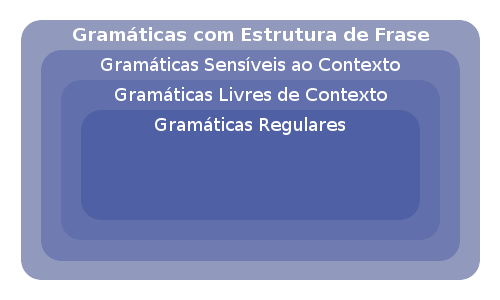
\includegraphics[scale=0.5]{driagrama_classes_gramaticas.png}
	\end{center}
	\legend{Fonte: Produzido pelo autor}
\end{figure}

Lembrando que as gramáticas são compostas por: um conjunto finito de símbolos não-terminais $N$, um conjunto finito de símbolos terminais $T$, um conjunto de produções $P$ e um símbolo inicial $\sigma$. A intersecção entre os conjuntos de símbolos não terminais e terminais deve ser vazia. O conjuto de produções é um subconjunto de todas as produções possíveis, o produto cartesiano de: todas as palavras geradas com símbolos não-terminais e terminais contendo pelo menos um símbolo não terminal (lado esquerdo da produção); todas as palavras geradas com símbolos não-terminais e terminais. O símbolo inicial deve pertencer ao conunto dos símbolos não terminais. Nas definições a seguir $\lambda$ denota a palavra nula.

\subsection{Gramáticas com Estrutura de Frase}
A gramática é com Estrutura de Frase se todas as produções são da forma:

$\alpha \to \delta$, onde $\alpha \in (N \cup T)$* - $T$*, $\delta \in (N \cup T)$*.

\subsection{Gramáticas Sensíveis ao Contexto}
A gramática é Sensível ao Contexto se todas as produções são da forma:

$\alpha A\beta \to \alpha \delta \beta$, onde $\alpha,\beta \in (N \cup T)$*$, A \in N, \delta \in (N \cup T)$* - \{$\lambda$\}.

\subsection{Gramáticas Livres de Contexto}
A gramática é Livre de Contexto se todas as produções são da forma:

$A \to \delta$, onde $A \in N, \delta \in (N \cup T)$*.

\subsection{Gramáticas Regulares}
A gramática é Regular se todas as produções são da forma:

$A \to a$ ou $A \to aB$ ou $A \to \lambda$.

\chapter{Rotação em árvores ordenadas}

\begin{figure}[H]
	\caption{\label{gram_cls}Diagrama sobre rotação de árvores binárias ordenadas}
	\begin{center}
	    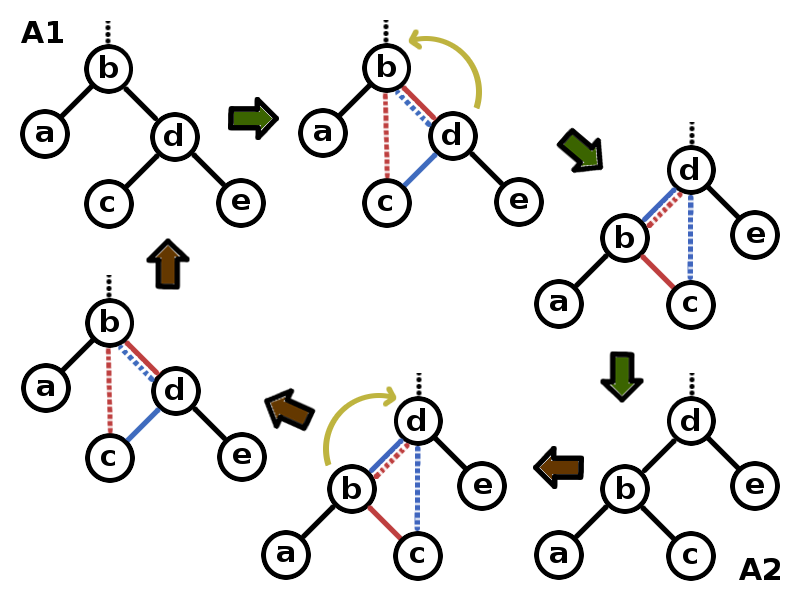
\includegraphics[scale=0.25]{tree_rotations.png}
	\end{center}
	\legend{Fonte: Produzido pelo autor}
\end{figure}

O diagrama contido na Figura 3 mostra graficamente como as rotações anti-horária e horária acontecem. A rotação anti-horária é explicada no fluxo representado através das setas verdes, que começa na árvore A1 e termina na árvore A2. A rotação horária de uma forma simétrica começa na árvore A2 e termina na árvore A1, as setas marrons representam o fluxo. As setas amarelas mostram o sentido das rotações executadas.

A rotação horária parte da árvore A2. A árvore seguinte mostra que o nó b, que inicialmente tem como filho direito o nó c, terá em seguida o nó d como seu filho direito. O filho esquerdo do nó d será alterado de nó b para nó c. A possível relação entre o nó d e o seu nó pai será passada para o nó b. Em seguida observamos como linhas contínuas as novas ligações e como tracejadas as antigas. Por fim chegamos a árvore A1 que é o resultado final da rotação horária sobre o nó d da árvore A2.

A rotação anti-horária é um processo simétrico à rotação horária. A sequência expressa através das setas verdes, de A1 até A2, explica a transformação da mesma forma como a sua transformação inversa explicada no tópico anterior sendo assim não será explicada em detalhes.

\chapter{Propriedades das operações}

\chapter{Números de Catalan}
Os números de Catalan é um conjunto de números que aparece em probelmas de enumeração de árvores como no problema de divisão dos polígonos de Euler. O $n$-ésimo número de Catalan pode ser obtido através da expressão $\frac{1}{n+1} \binom{2n}{n} $ \cite{wolfram}. Os dez primeiros números da sequência, começando com $n = 0$, são: 1, 1, 2, 5, 14, 42, 132, 429, 1430, 4862.

Os números de Catalan aparecem em diversos problemas, entre eles o problema das Ordens de Mutiplicação.
Este problema se refere a uma sucessão de $n$ multiplicações onde a ordem dos $n+1$ operandos não pode ser alterada. De acordo com a expressão apresentanda anteriormente a solução é o n-ésimo elemento do conjunto dos números de Catalan \cite{catNum}.

% ---

% ----------------------------------------------------------
% PARTE
% ----------------------------------------------------------
\part{Experimento}
O experimento desenvolvido neste trabalho consiste na criação de um jogo educacional utilizando a tecnologia HTML5. Como tecnologias complementares foram utilizadas: Javascript, CSS3, Queue.js, Highcharts e PhoneGap. O conteúdo educacional escolhido para ser trabalhado no jogo foi expressões algébricas. O jogo consiste em apresentar uma expressão ao jogador e pedir para que ele selecione e resolva cada uma das operações até chegar ao resultado final.

\chapter{Visão geral do fluxo}
O fluxo tem início quando o usuário acessa o jogo – como página de internet ou aplicativo para dispositivo móvel. O jogo inicializa e apresenta o botão “Play” para que o jogador comece os testes. Quando iniciados os testes o jogo escolhe uma expressão e a apresenta ao usuário para que ele selecione uma operação para resolver.

Assim que uma operação é selecionada o programa avalia se esta pode ser resolvida e apresenta a pontuação. Caso a operação selecionada não possa ser resolvida o programa se mantém no estado de seleção, no caso contrário o programa pede a solução para a operação selecionada. Depois que o usuário passa a solução o jogo apresenta a pontuação. Se a solução passada estiver incorreta o jogo permanece no estado de resolução, se a solução estiver correta a aplicação apresenta a expressão resultante.

Enquanto houver operações não resolvidas o fluxo se repete desde a seleção de operação. Quando não houver mais operações a serem resolvidas o programa apresenta os botões “Next...” e “Exit” para o jogador fazer o próximo teste ou sair do jogo respectivamente. Se o jogador for para o próximo teste o fluxo volta para o passo de escolha de expressão, no caso do jogador sair o programa apresenta a tela final.

\section{Inicialização da aplicação}
A função start é responsável pela inicialização da aplicação, recebe como parâmetro o identificador do elemento HTML que irá conter a tela do jogo e insere os principais elementos HTML do jogo, inclusive a tela inicial para que o usuário possa iniciar o jogo.

\section{Escolha da expressão}
A escolha da expressão é feita através da função newXp. Inicialmente a rotina seleciona uma expressão, escolhendo uma das disponibilizadas através do método startDB (executado no início dos testes) ou gerando uma com a função makeExp. Em seguida a expressão selecionada é passada para o contexto do jogo junto de suas soluções.

A criação de novas expressões leva em conta duas variáveis: número de operações e um conjunto de possíveis operações a serem utilizadas. As expressões são criadas de forma aleatória. A probabilidade para cada operação ser sorteada é 1 em n, onde n é o tamanho do conjunto de operações passado. 	Não existe restrição de unicidade para o conjunto de operações que são passadas para a função makeExp possibilitando alterar a probabilidade de que uma determinada operação seja escolhida.

Caso a expressão escolhida tenha sido gerada a fase de passar a expressão para o contexto do jogo envolve a avaliação da expressão para conhecer todas as soluções possíveis para a expressão. A avaliação da expressão é feita através de um algoritmo iterativo implementado na função evaluateTreeIt.

\section{Apresentação da expressão}
A expressão é apresentada utilizando a função appendXp que recebe como parâmetro a expressão e a imprime na tela utilizando a função htmlfy, uma função recursiva que retorna os elementos HTML que representam visualmente a expressão.

\section{Selecão da operação}
A seleção da operação é acionada através de um clique simples com o botão esquerdo do mouse ou toque (no caso de dispositivos móveis) sobre a operação. A função opClick é responsável por tratar tais eventos recebendo como parâmetro o identificador da operação. Internamente a função opClick faz uso da função select que é responsável por avaliar se a operação pode ou não ser resolvida.

\section{Pontuação}
Sempre que houver uma seleção ou tentativa resolver uma operação o jogo avalia se a ação está correta e então apresenta a pontuação através da função spanWarn que recebe como parâmetros o tipo de pontuação, perda ou ganho, e o respectivo valor.

Quando o jogador acerta uma seleção ou resolução na primeira tentavia ele recebe 1 ponto inteiro. Para cada erro o ponto é divido ao meio, assim que se o acerto ocorrer na segunda tentativa o jogador recebe meio ponto. A seleção da última operação não é pontuada por ser uma opção única.

\section{Pedido de solução}
Sempre que uma operação for selecionada corretamente o jogo pede ao usuário a solução através da função askForSolution que apresenta ao usuário a operação isolada seguida de uma caixa de texto, para que o usuário insira a solução daquela operação. Os elementos HTML apresentados contém aqueles retornados pela função htmlfy.

\section{Passagem da solução}
Depois que o usuário inserir a solução na caixa de texto e apertar a tecla ENTER ou tirar o foco da caixa de texto o programa faz uma avaliação da solução passada através da função solSubmit. Caso a solução esteja correta a caixa de texto é transformada em texto simples. Se houver mais de uma possível solução apenas aquela que foi resolvida permanece na tela, as outras são eliminadas da tela.

\section{Exemplo}
O exemplo a seguir exemplifica como o fluxo do jogo é percebido pelo usuário através da interface. Após inicializar a aplicação o usuário vê a tela inicial e o botão “Play”. Após apertar o botão “Play” o jogo apresenta uma expressão para o jogador resolver.

\begin{figure}[H]
	\caption{\label{xp_1} O sistema apresenta a expressão a ser resolvida}
	\begin{center}
	    
\includegraphics[scale=1]{xp_4_1.png}
	\end{center}
	\legend{Fonte: Produzido pelo autor}
\end{figure}

O jogador seleciona uma operação que não pode ser resolvida e perde metade da pontuação da seleção.

\begin{figure}[H]
	\caption{\label{miss_0_5_1}Jogador perde metade da pontuação da seleção}
	\begin{center}
	    
\includegraphics[scale=1]{miss_0_5.png}
	\end{center}
	\legend{Fonte: Produzido pelo autor}
\end{figure}

Em seguida o usuário seleciona a uma operação que pode ser resolvida e ganha a pontuação da seleção.

\begin{figure}[H]
	\caption{\label{score_0_5_1}Jogador ganha a pontuação da seleção}
	\begin{center}
	    
\includegraphics[scale=1]{score_0_5.png}
	\end{center}
	\legend{Fonte: Produzido pelo autor}
\end{figure}

O programa então apresenta a operação isolada e a caixa onde o usuário insere a solução. Este passo será omitido no resto do exemplo.

\begin{figure}[H]
	\caption{\label{xp_2}Programa pede a solução da operação}
	\begin{center}
	    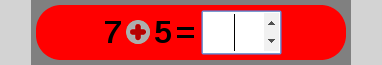
\includegraphics[scale=1]{xp_4_2_asksol_1.png}
	\end{center}
% 	\legend{Fonte: Produzido pelo autor}
\end{figure}

O jogador erra a solução e perde metade da pontuação da resolução.

\begin{figure}[H]
	\caption{\label{xp_3}O usuário insere um valor errado como solução}
	\begin{center}
	    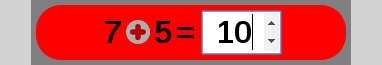
\includegraphics[scale=1]{xp_4_3_wrongans_1.png}
	\end{center}
	\legend{Fonte: Produzido pelo autor}
\end{figure}

\begin{figure}[H]
	\caption{\label{miss_0_5_2}O jogador perde metade dos pontos da solução}
	\begin{center}
	    
\includegraphics[scale=1]{miss_0_5.png}
	\end{center}
	\legend{Fonte: Produzido pelo autor}
\end{figure}

Em seguida o valor é corrigido e o usuário ganha a pontuação da solução.

\begin{figure}[H]
	\caption{\label{xp_4}O jogador insere a solução correta}
	\begin{center}
	    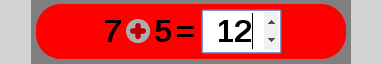
\includegraphics[scale=1]{xp_4_4_rightans_1.png}
	\end{center}
	\legend{Fonte: Produzido pelo autor}
\end{figure}

\begin{figure}[H]
	\caption{\label{score_0_5_2}O sistema pontua o jogador pela solução}
	\begin{center}
	    
\includegraphics[scale=1]{score_0_5.png}
	\end{center}
	\legend{Fonte: Produzido pelo autor}
\end{figure}

O campo de texto é transformado em texto simples e a expressão resultante é apresentada ao usuário. O fluxo seleção/resolução se repete.

\begin{figure}[H]
	\caption{\label{xp_5}O sistema mostra a expressão resultante}
	\begin{center}
	    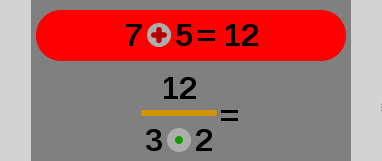
\includegraphics[scale=1]{xp_4_5.png}
	\end{center}
	\legend{Fonte: Produzido pelo autor}
\end{figure}

\begin{figure}[H]
	\caption{\label{score_1_1}O jogador recebe 1 ponto pelo acerto da seleção}
	\begin{center}
	    
\includegraphics[scale=1]{score_1.png}
	\end{center}
	\legend{Fonte: Produzido pelo autor}
\end{figure}

A divisão pode ser resolvida de duas maneiras e o jogo apresenta as duas possibilidades de solução.

\begin{figure}[H]
	\caption{\label{xp_7}O jogo aparesenta duas possibilidades de resolução para a divisão}
	\begin{center}
	    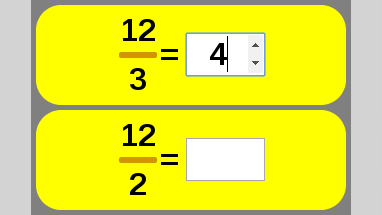
\includegraphics[scale=1]{xp_4_7_rightans_2.png}
	\end{center}
	\legend{Fonte: Produzido pelo autor}
\end{figure}

\begin{figure}[H]
	\caption{\label{score_1_2}O jogador recebe 1 ponto pelo acerto da solução}
	\begin{center}
	    
\includegraphics[scale=1]{score_1.png}
	\end{center}
	\legend{Fonte: Produzido pelo autor}
\end{figure}

O fluxo seleção/resolução se repete.

\begin{figure}[H]
	\caption{\label{xp_8}A nova expressão é apresentada ao usuário}
	\begin{center}
	    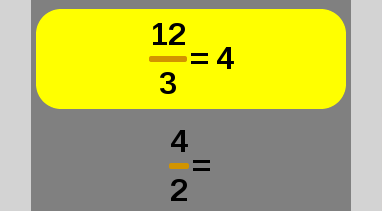
\includegraphics[scale=1]{xp_4_8.png}
	\end{center}
	\legend{Fonte: Produzido pelo autor}
\end{figure}

A seleção da última operação não é pontuada.

\begin{figure}[H]
	\caption{\label{score_0_1}A seleção da última operação não é pontuada}
	\begin{center}
	    
\includegraphics[scale=1]{score_0.png}
	\end{center}
	\legend{Fonte: Produzido pelo autor}
\end{figure}

\begin{figure}[H]
	\caption{\label{xp_10}O jogador insere a última solução a que está correta}
	\begin{center}
	    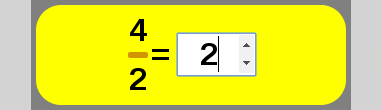
\includegraphics[scale=1]{xp_4_10_rightans_3.png}
	\end{center}
	\legend{Fonte: Produzido pelo autor}
\end{figure}

\begin{figure}[H]
	\caption{\label{score_1_3}O jogador recebe a pontuação referente a solução}
	\begin{center}
	    
\includegraphics[scale=1]{score_1.png}
	\end{center}
	\legend{Fonte: Produzido pelo autor}
\end{figure}

	Não existem mais operações para serem resolvidas e as opções de continuar ou sair são apresentadas ao usuário.
	
\begin{figure}[H]
	\caption{\label{xp_11}A tela final é apresentada}
	\begin{center}
	    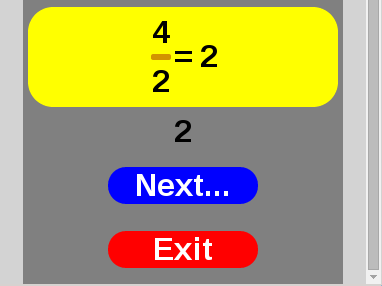
\includegraphics[scale=1]{xp_4_11.png}
	\end{center}
	\legend{Fonte: Produzido pelo autor}
\end{figure}

\chapter{Criação de expressões}

As expressões algébricas utilizadas são linguagens formais pois são um subconjunto de todas as palavras existentes para um determinado alfabeto. Para tanto existe pelo menos uma gramática capaz de gerar a linguagem formal envolvida.

\subsection{A linguagem formal envolvida no jogo}
Vamos partir do conjunto de símbolos terminais que deve conter: as operações de soma, subtração, multiplicação e divisão; um conunto de números dado por um intervalo fechado sobre o conjunto dos inteiros; parênteses. Logo temos T = {+, -, *, /, -2, -1, 0, 1, 2, (, )}. Escolhemos um pequeno intervalo de inteiros neste caso para manter o conjunto pequeno.

	As expressões que fazem da linguagem formal envolvida são do tipo infixa, ou seja, a operação é posicionada no meio de dois elementos que podem ser outras uma outra operação ou um inteiro. Esta escolha se dá por ser o formato que os alunos estão acostumados a ver.
	
\subsubsection{Prefixo, infixo, pósfixo}
Podemos representar uma operação matemática utilizando os três seguintes formatos: prefixo, infixo e pósfixo. No primeiro formato a operação é posicionada em primeiro, antes dos dois operandos. O formato pósfixo é simétrico ao formato anterior, ou seja, a operação é posicionada em último depois dos operandos. Uma vantagem da utilização dos formatos anteriores é a não necessidade de utilizar parênteses para expressar precedência entre as operações. Já no formato infixo a operação é posicionada entre os operandos e necessita utilizar parênteses para expressar precedência entre as operações.

\subsubsection{Parênteses}
A necessidade de utilizar parênteses para expressar precedência entre operações na forma infixa não ocorre para todas as operações na expressão. Os casos são os seguintes: quando uma subtração tem como operando direito outra operação que seja uma soma ou subtração; quando o operando de uma multiplicação ou divisão for uma operação de soma ou subtração; quando um número negativo é operando direito de uma operação.

\subsubsection{Gramática referência}
Tendo em conta os pontos apresentados anteriormente é possível criar uma gramática que seja capaz de gerar as expressões que serão utilizadas no jogo. Algumas simplificações serão feitas a seguir nas produções. Os terminais o e i representam os seguintes conjuntos de terminais respecitvamente o conjunto das operações evolvidas e o conjunto expresso por um intervalo fechado  e contínuo sobre os números inteiros.

	Com a simplificação anterior não existe necessidade de criar uma regra de produção para cada operação e para cada inteiro. Subentende-se que estes terminais, que representam conjuntos, poderiam se desdrobrar em um símbolo não-terminal que produz cada um dos elementos do conjunto que representam sozinho.
	
	A gramática pensada como referência para a solução adotada na criação das expressões é a seguinte:
	
$G: (N, T, P, S)$, onde:

$N = \{S,E\}$,

$T = \{o,i,(,)\}$,

$P$ é o conjunto das seguintes produções:

$S \to (EoE)$

$E \to (EoE) | (i)$,

$\sigma = S$.

Note que a linguagem possui parênteses para todas as operações e inteiros. A linguagem foi pensada assim pois a forma ecolhida para representar suas palavras não foi um texto simples mas sim uma árvore que por natureza já expressa as precedências entre as operações além da necessidade dos parênteses para alguns números inteiros negativos. A lógica de apresentação de parênteses está encapsulada na função htmlfy.

	De acordo com a Classificação de Chomsky, apresentada anteriormente, tal gramática é Livre de Contexto.
	
\subsection{Algoritmo para criação de expressões}
No código Javascript contido no arquivo xpress.js temos a função makeExp responsável pela criação das expressões. A função recebe como parâmetros o número de operações que a expressão deve conter e um conjunto contendo quais operações deversão fazer parte da expressão. A lógica da função makExp está encapsulada em duas funções, makeOps e fillWithInts, onde a primeira gera uma árvore de operações apenas e a segunda preenche a árvore com inteiros, lembrando que a árvore utilizada para representar as expressões é do tipo binária já que cada operação possui dois operandos.

\subsubsection{makeOps}
A função makeOps tem os mesmos parâmetros da função makeExp. Caso as operações não sejam passadas a função utiliza todas as operações (soma, subtração, multiplicação e divisão). A rotina começa com a criação de: uma lista de possíveis operações pai iniciada vazia; uma referência para a raíz da árvore de operações que começa com o valor nulo.

	O passo seguinte é uma iteração sobre o número de operações a serem criadas. Uma operação daquelas passadas como parâmetro é sorteada e passada como parâmetro para a função criadora dos nós que retorna um nó com aquela determinada operação. Se a referência a raíz feita fora da iteração ainda possuir o valor nulo a referência apontará então para o nó criado. No caso contrário o programa sorteia um possível pai da lista, remove da mesma, definindo este como pai do nó criado. 
	
	No final da iteração o programa adiciona novas entradas na lista de possíveis pais. Estas entradas representam a ideia de que o ultimo nó criado pode ser pai a esquerda e pai a direita. Quando não existem mais iterações para acontecer a função retorna o nó referenciado como raíz.
	
\subsubsection{fillWithInts}
No caso de uma árvore incompleta, ou seja, existe pelo menos um operando de uma operação que não foi definido a função fillWithInts pode torná-la completa. A função recebe como parâmetro a raíz da árvore a ser preenchida com inteiros. A função faz uma busca em profundida na árvore para encontrar todas as operações que possuem operandos não definidos e então os define.

	A busca em profundidade é feita utilizando uma pilha de nós a serem analisados. A pilha começa com a raíz que foi passada como parâmetro. Enquanto houver nós na pilha o programa tira o último nó da pilha testando se seus operandos, esquerdo e direito, são nós ou se estão vazios. No caso de o operando ser uma operação o programa o empilha para ser futuramente analisado, se não a rotina cria um nó com um número inteiro e o define como o operando que falta.
	
\subsubsection{Restrição}
Embora o algoritmo criado seja capaz de criar expressões com todas as operações (soma, subtração, multiplicação e divisão) no experimento este é utilizado somente para criar expressões com somas e subtrações, as duas com a mesma probabilidade.

	A restrição foi feita para limitar o escopo deste trabalho pois como requerimento todos os números envolvidos nas expressões, inclusive aqueles que são a solução de uma operação, devem ser inteiros. Neste caso se as expressões possuem divisão o algoritmo na expressão fillWithInts deveria levar tal fato em conta e garantir que os resultados das divisões sejam números inteiros.
	
\section{Análise de soluções}
As expressões algébricas envolvidas no experimento podem ter mais de uma forma de solução e para que o jogo possa avaliar corretamente a resolução da expressão feita pelo usuário é necessário fazer a avaliação da expressão a fim de encontrar todas as ordens de resolução possível.

\subsection{Ambiguidade}
A possibilidade de mais de uma solução para uma mesma expressão se dá pelo fato de que esta expressão pode ser gerada de mais de uma forma utilizando as produções. Por exemplo, 3+4+5 é uma expressão ambigua pois existem duas árvores que podem representá-la:

ARVORE
     
Como vemos a precedência entre as operações varia de uma árvore para a outra. Na primeira a operação 3+4 não tem nenhuma dependência e pode ser resolvida, na segunda isto ocorre com a operação 4+5. A transformação que explica a mudança da primeira árvore para a segunda é uma rotação no sentido horário feita na raíz da árvore. A possibilidade da rotação no sentido horário se dá pois não existe precedência real entre as operações envolvidas significando que as duas podem ser resolvidas no primeiro passo de resolução.

	A rotação utilizada não muda o significado da expressão. Tal fato também ocorre em árvores binárias ordenadas as quais podem ter seus nós rotacionados indeterminadamente sem perder a ordenação de seus elementos. Embora exista tal semelhança as árvores que respresentam as expressões neste experimento não podem ser rotacionadas livremente sem que o significado se altere.
	
	A subtração de uma soma é um caso onde a rotação das operações não pode ocorrer. Por exemplo, 5-(4+3). Existe uma precedência lógica nesta expressão que representa a necessidade de primeiro somar para depois subtrair. A árvore que representa tal expressão é esta:
	
ARVORE
           
A lógica que explica a utilização dos parênteses em operações é a mesma lógica que explica  a possibilidade de rotação na árvore sem perder o significado, ou seja, como a soma é o operando direito da subtração esta deve estar entre parênteses e por sua vez a subtração não pode ser rotacionada no sentido. Além da lógica anterior que explica os parênteses a rotação só pode ocorrer se o nó a ser rotacionado e aquele que toma o seu lugar são operações.

\subsection{Rotação das árvores}
Como mencionado anteriormente as árvores podem ser rotacionadas tanto no sentido horário como no sentido anti-horário. A lógica que explica a possibilidade de rotação varia entre a rotação horária e a anti-horária já que a consideração que deve ser feita em relação a subtração ocorre apenas quando tentamos fazer uma rotação anti-horária (como no caso anterior da expressão 5-(4+3)).


\subsubsection{Rotação horária}
	A rotação neste sentido é sempre possível para as operações que possuem como filho esquerdo outra operação, já que a única restrição a ser considerada para saber se a rotação pode ser feita se refere apenas ao filho direito do nó a ser rotacionado.
	
\subsubsection{Rotação anti-horária}
	A rotação anti-horária não pode ser feita para toda operação que tem como filho direito outra operação, a operação pai em questão não pode ser uma subtração.
	
\subsection{Números de Catalan}
Como mostrado por Robert Sedgewick e Phillipe Flajolet (2013) os números Catalãos explicam o número de possíveis árvores binárias ordenadas de acordo com o número de nós internos da árvore inicial. O teorema Enumeração de Árvores Binárias enuncia: “O número de árvores binárias com N nós internos e N+1 nós externos é dado pelos números Catalãos” (Robert Sedgewick e Phillipe Flajolet, 2013).

	No caso do experimento algumas rotações não são possíveis nas expressões e sendo assim temos como valor máximo para o tamanho do conjunto das possíveis árvores o número Catalão associado ao número de nós internos na árvore. No entanto se dividirmos as árvores aonde existem as retrições de giro, subtrações com operações como filho direito, podemos encontrar o número de possíveis árvores. Depois de dividir a árvore nos pontos de restrição fazemos a análise para cada árvore resultante e multiplicamos os números para encontrar o número de possíveis árvores.
	
\subsection{Algoritmo para análise de soluções}
A criação de expressões é um ponto importante no experimento desenvolvido neste tabalho pois evita a necessidade da criação manual de expressões e cria um potencial repositório infinito de expressões. Para tanto é necessário que a aplicação seja capaz de avaliar a expressão criada para encontrar todas as soluções possíveis.

	O algoritmo utilizado para a análise de soluções analisa a árvore que representa a expressão dos nós mais distantes da raíz até os mais próximos. Desta forma cada nó pai conhece todas as transformações possíveis para seus nós filhos. A partir do produto cartesiano de todas as transformações possíveis o nó é testado para rotações sobre todas as transformações contidas no produto cartesiano de soluções dos filhos.
	
	Quando o nó a ser avaliado for raíz o algoritmo testa para conhecer se as soluções avaliadas já existem em um conjunto final de soluções ou não, caso não o algoritmo adiciona tal soluções a este conjunto.
	
	Caso uma nova solução seja encontrada esta é colocada em uma fila para que seja analisada em seguida, assim como a árvore inicial foi. O pseudo-código a seguir explica em mais detalhes o funcionamento do algoritmo para uma dereminada árvore:
	
novo Mapa Soluções;
adicionar árvore a Soluções;
nova Fila Soluções a avaliar;
enfilar árvore em Soluções a avaliar;
enquanto Soluções a avaliar não é vazia {
	nova Solução S1;
	tirar a primeira Solução da fila e atribuir à S1;
	transformar arvore utilizando as transformações de S1;
	nova Lista Nós a avaliar;
	criar Lista de nós para a raíz de S1 e atribuir à Nós a avaliar;
	novo Mapa Soluções por nó;
	para cada Nó N em Nós a avaliar {
		Soluções por nó recebe uma nova Lista em N;
		nova Lista Pré-soluções;
		combinar soluções dos filhos direito e esquerdo de N
			e atribuir a Pré-soluções;
		para cada Solução P em Pré-soluções {
			nova Solução S2 recebe a combinação de S1 e P;
			adicionar S2 à Lista no Soluções por nó em N;
			se N é raiz e a chave de S2 não está em Soluções {
				adicionar S2 a Soluções e Soluções a avaliar;
			}
			novo Nó H recebe N;
			nova Solução SH recebe S2;
			enaquanto H pode ser rotacionado no sentido horário {
				rotacionar H no sentido horário;
				adicionar transformação feita às transformações de SH;
				adicionar SH à Lista no Soluções por nó em N;
				se o pai de H é raiz e a chave de SH não está em Soluções {
					adicionar SH a Soluções e Soluções a avaliar;
				}
				atribuir o pai de H a H;
			}
			desfazer todas as rotações feitas no sentido horário;
			novo Nó AH recebe N;
			nova Solução SAH recebe S2;
			enaquanto AH pode ser rotacionado no sentido anti-horário {
				rotacionar AH no sentido anti-horário;
				adicionar transformação feita às transformações de SAH;
				adicionar SAH à Lista no Soluções por nó em N;
				se o pai de AH é raiz e a chave de SAH não está em Soluções {
					adicionar SAH a Soluções e Soluções a avaliar;
				}
				atribuir o pai de AH a AH;
			}
			desfazer todas as rotações feitas no sentido anti-horário;
			desfazer as transformações de P;
		}
	}
	desfazer as trasnformações de S1;
}	

\subsection{Desempenho do algoritmo}
Para testar o desempenho do algoritmo de avaliação de expressões a função evaluateTreeItTest foi criada. A função recebe quatro parâmetros de teste. Os dois primeiros são os limites de um intervalo de números inteiro que representam os tamanhos de árvores a serem testadas. O parâmetro seguinte se refere ao número de testes por tamanho de árvore. O ultimo parâmetro é opcional, uma lista de possíveis operações a serem utilizadas na criação das expressões que serão testadas.

	Nos gráficos a seguir podemos observar os resultados dos testes. Os teste foram feitos 10 vezes para árvores de 3 a 9 nós, onde no primeiro teste somente operações de soma foram utilizadas diferente so segundo que também utiliza subtrações.
	
\begin{figure}[H]
	\caption{\label{gram_cls}Diagrama sobre rotação de árvores binárias ordenadas}
	\begin{center}
	    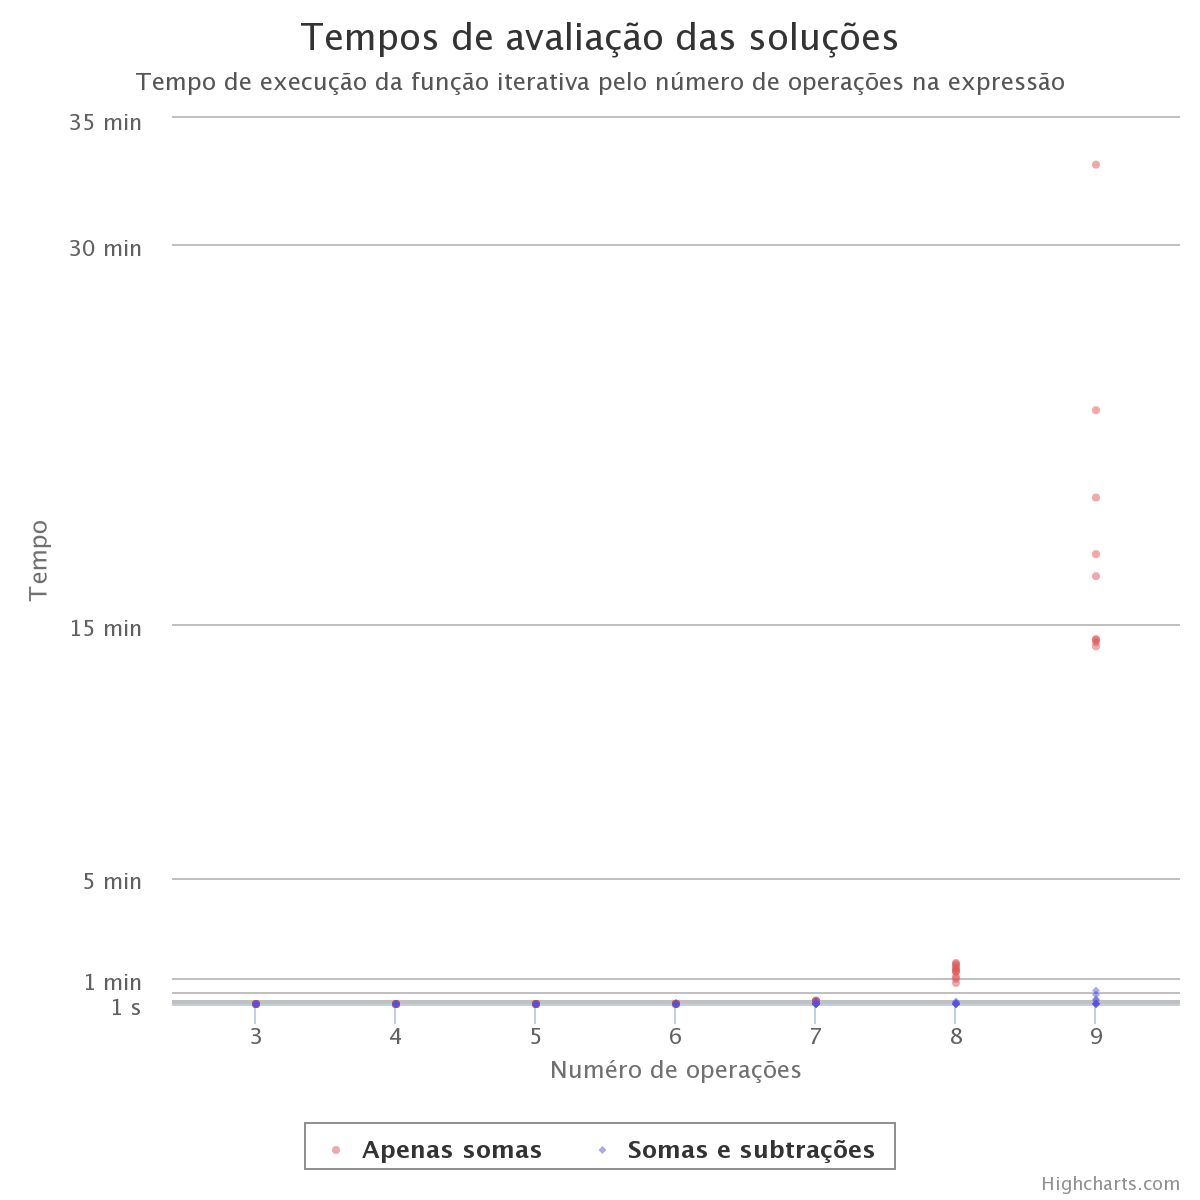
\includegraphics[scale=0.25]{timming_test_lin.png}
	\end{center}
	\legend{Fonte: Produzido pelo autor}
\end{figure}

\begin{figure}[H]
	\caption{\label{gram_cls}Diagrama sobre rotação de árvores binárias ordenadas}
	\begin{center}
	    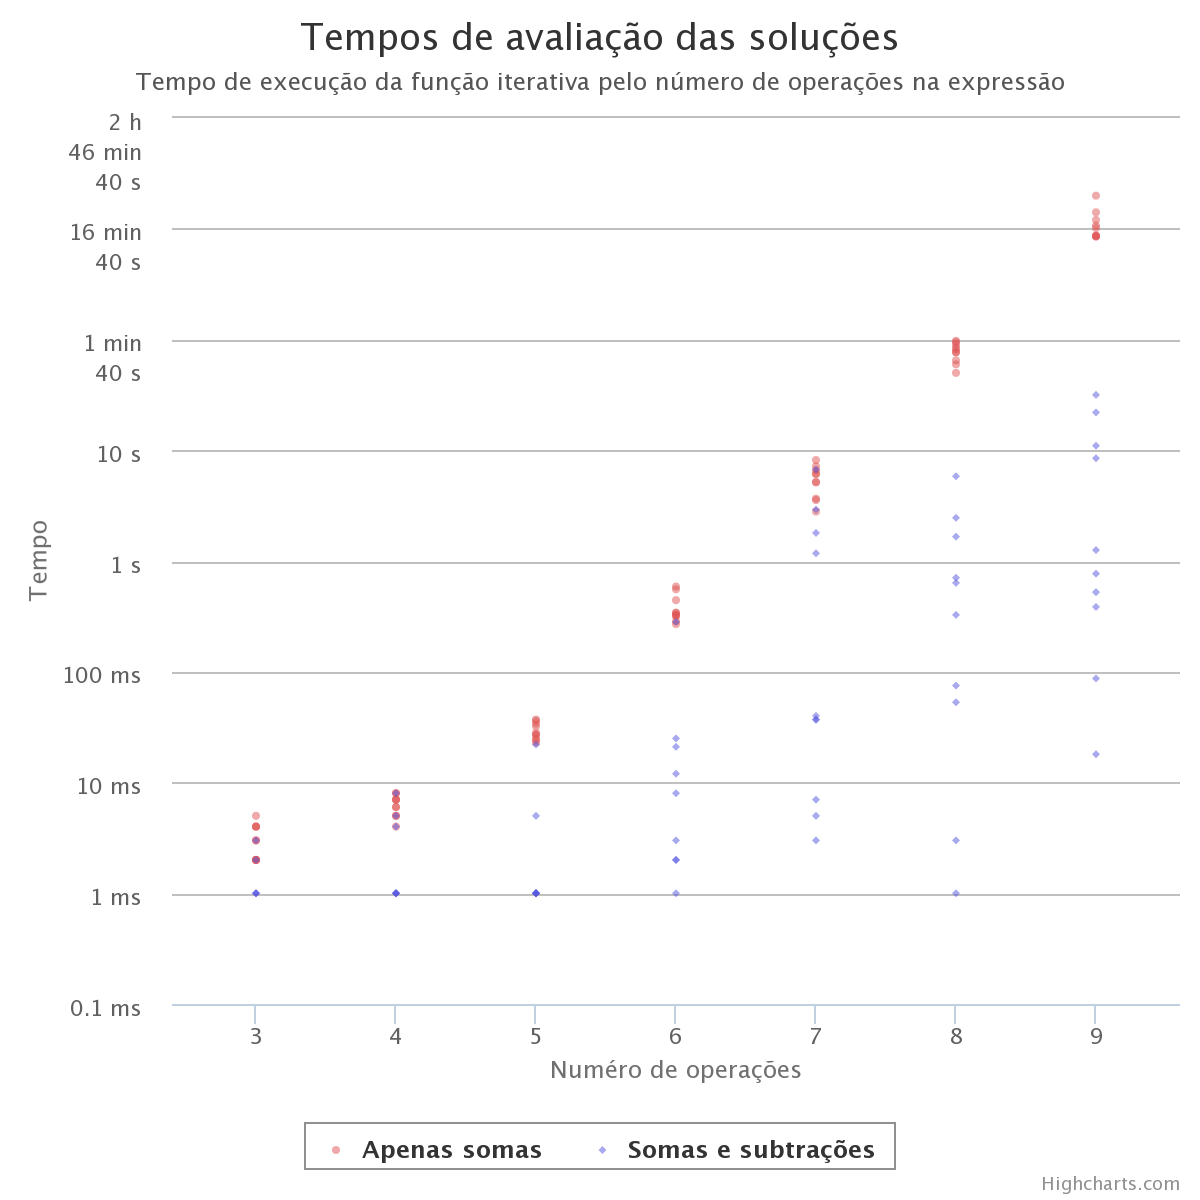
\includegraphics[scale=0.25]{timming_test_log.png}
	\end{center}
	\legend{Fonte: Produzido pelo autor}
\end{figure}

A diferença nos tempos das séries sem e com soma se devem ao fato de que expressões com subtração tem limitações de rotação. O primeiro gráfico em escala linear mostra o comportamento exponencial da expressão. No gráfico cuja a escala é logarítmica podemos observar com maior clareza como as tempos nas expressões que envolvem subtração variam em um intervalo cujo tempo máximo é o tempo para as árvores que não envolvem subtrações. Isto se deve ao caráter aleatório do algoritmo de geração de expressões. Uma expressão só com somas pode ser gerada mesmo no teste que envolve também subtrações.

\section{Modelo e estruturas de dado}
Por mais que o experimento não utilize uma aplicação de banco de dados existe um modelo de dados intrínseco expresso no diagrama a seguir.

\begin{figure}[H]
	\caption{\label{gram_cls}Diagrama sobre rotação de árvores binárias ordenadas}
	\begin{center}
	    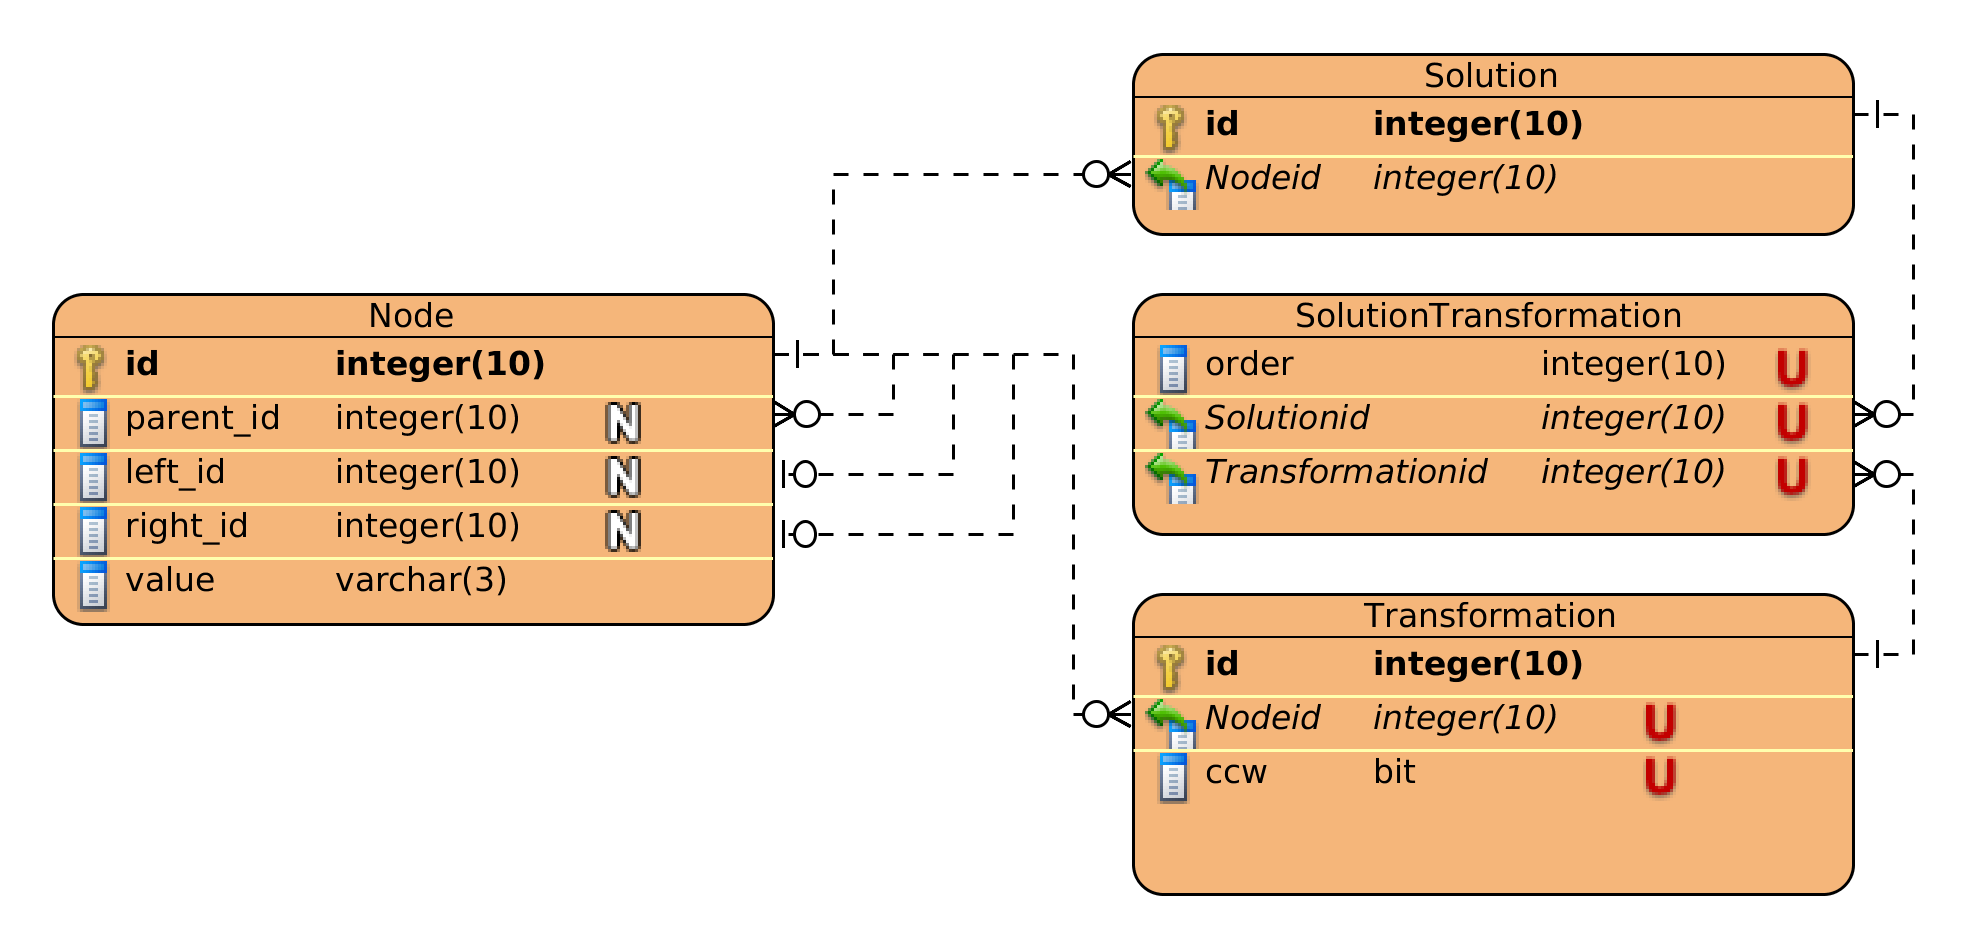
\includegraphics[scale=0.5]{datamodel.png}
	\end{center}
	\legend{Fonte: Produzido pelo autor}
\end{figure}

O diagrama representa as expressões e suas respectivas soluções. Como a estrutura de dados escolhida para representar as expressões foi a árvore, as expressões são armazenadas podem ser armazenadas da mesma forma. Cada nó (Node) aponta para o seu nó pai e seus nós filhos.

As soluções (Solution) para uma determinada expressão são armazenadas na forma de uma lista ordenada de transformações (Transformation). A lista de ordenada de transformações é representada através da entidade SolutionTransformation.


% ----------------------------------------------------------
% PARTE
% ----------------------------------------------------------
\part{Tecnologias}
% ----------------------------------------------------------

% ---
% primeiro capitulo de Resultados
% ---
\chapter{HTML5}
De acordo com o texto de introdução de W3SCHOOLS HTML5 é o padrão HTML mais recente. A versão anterior (4.01) foi lançada em 1999 e como a internet mudou significantemente desde então a versão 5 vem para substituir a versão 4.01, além do XHTML e o HTML DOM Level 2. A nova versão provê de animações a gráficos, musicas a filmes além de possibilitar aplicações web complexas. O padrão HTML5 é multiplataforma e é feito para funcionar em PCs, Tablets, Smartphones e Smart TVs.

	A versão 5 do padrão HTML é uma cooperação entre o World Wide Web Consortium (W3C) e o Web Hypertext Application Tecnology Working Group (WHATWG). Ambas as organizações trabalhavam em diferentes aspectos de aplicações web e em 2006 resolveram se juntar para criar a nova versão do HTML. Algumas diretrizes foram estabelecidas para o futuro empreendimento \cite{htmlInt}:

\begin{alineas}

\item Novas funcionalidades devem estar baseadas em HTML, CSS, DOM e JavaScript;

\item A necessidade de plugins externos deve ser reduzida;

\item Lidar com erros deve ser mais fácil que nas versões anteriores;

\item “Scripting” deve ser substituido por mais marcações;

\item O padrão deve ser independente de dispositivo;

\item O publico deve ter visibilidade do processo de desenvolvimento

\end{alineas}

Entre as novas “features” disponibilizadas na nova versão temos:

\begin{alineas}

\item O elemento canvas para desenho em 2D;

\item Os elementos video e audio para execução de mídias;

\item Suporte para armazenamento local

\end{alineas}

\section{O surgimento do HTML}
A World Wide Web teve inicio no CERN, Laboratório para Física de Particulas em Geneva, Suiça. O conceito do HTML surgiu enquanto Tim Berners-Lee trabalhava em uma seção de serviços computacionais do CERN. Tim teve a ideia de permitir que pesquisadores em diferentes lugares do mundo pudessem organizar e juntar informações remotamente, já que as pesquisas em Física de Particulas envolve com frequência diversos institutos de varios lugares do mundo. A questão não era apenas disponibilizar um grande número de pesquisas mas permitir que ligações entre os documentos fossem estabelecidas. Antes de trabalhar no CERN Tim havia trabalhado com produção de documentos e processamento de texto. Tim pensou que a solução seria desenvolvida como uma forma de hipertexto.

O protótipo de navegador web estava pronto em 1990 para o computador NeXT e foi desenvolvido por Tim Berners-Lee. O surgimento da web no começo dos anos 90 está relacionado aos desenvolvimentos em tecnologias de comunicação durante o período assim como o hipertexto ganhava espaço e comçava a ser usado em computadores. O sistema de nomes de domínios (DNS) também foi importante no surgimento da Web pois facilitava o acesso às máquinas específicas.

Tim Berners-Lee via a viabilidade dos links globais de hipertexto. Uma consideração importante feita por Tim foi a importância de que tal hipertexto deveria funcionar nos mais diversos computadores que estavam ligados à Internet. Tim desenvolve um software e um protocolo (HTTP), que eram capazes de recuperar documentos de texto utilizando links de hipertexto, para demonstrar sua forma de publicar documentos. O texto que era utilizado pelo protocolo HTTP (HyperText Transfer Protocol) foi nomeado de HTML que significa linguagem de marcação de hipertexto (HyperText Mark-up Language).

A linguagem HTML criada por Tim Berners-Lee se baseou em um método de marcação de textos que organizava o texto em unidades estruturais como parágrafos, cabeçalhos entre outras, o SGML que era um método acordado internacionalmente. SGML significa linguagem padrão generalizada de marcação (SGML). Tal embasamento foi um fator que colaborou para o sucesso da ideia de Tim \cite{htmlHist}.

\section{A evlução do padrão HTML}
O HTML 2, nomeado assim por Tim Berners-Lee, surgiu para resolver o problema da linguagem que estava se tornando mal-definida conforme diversos navegadores adicionavam novos elementos HTML de uma forma não coordenada. Para tanto Dan Connolly e seus colegas fizeram o trabalho de unir as diferentes variantes e colocar em um documento de rascunho. Feito o rascunho este foi circulado pela Internet para que a comunidade pudesse comentar. O resultado de tal esforço foi a especificação da nova versão do HTML.

A dificuldade em manter o padrão não foi resolvida de fato na versão 2. O HTML 3, que foi publicado como um rascunho em 1995, também sofreu a dificuldade de manter o padrão da linguagem. O rascunho muito longo teve dificuldades em ser ratificado pelo IETF devido ao tamanho do esforço estimado. O problema em manter o padrão era semelhante ao enfrentado antes da especificação, cada navegador implementava diferentes subconjuntos do padrão além de possíveis extensões à linguagem. O HTML 3 não se tornou de fato um padrão.

Por mais que o HTML 3 não se tornou padrão o rascunho fez progressos importantes lidando com tabelas, notas de rodapé, formulários além de incluir o elemento STYLE e o atributo CLASS para encorajar os autores utilizarem estilo em seus documentos. Ainda em 1995 foi apresentado o artigo sobre a internacionalização da Web que previa acabar com a restrição de cunjunto de caracteres para que outros além do Latin-1 pudessem ser utilizados.

A especificação do HTML 3.2 foi endossada em janeiro de 1997 pelo W3C (World Wide Web Consortium) e trazia como um dos novos elementos disponíveis o OBJECT para incorporar objetos, por exemplo applets, dentro de um documento HTML. O HTML 3.2 foi resultado de uma combinação de todas as especificações anteriores e foi amplamente aprovada. \cite{htmlHist}

A versão anterior a especificação 5 é o HTML 4.01, revisão do HTML 4. Entre as diversas melhorias temos mecanismos para folhas de estilo, scripting e quadros. A versão 4 foi desenvolvida com ajuda de experts em internacionalização. A incorporação do RFC2070 realizou a internacionalização do HTML \cite{html4Int}.

\chapter{Tecnologias complementares}

\section{Highcharts}
Highcharts é uma API Javascript utilizada para gerar gráficos em páginas HTML. Os gráficos possuem varias opções de configuração o que os tornam muito flexíveis. A biblioteca Javascript é capaz de gerar diversos tipos de gráficos como: linha, área, coluna, pizza, dispersão, relógio. A API é bastante documentada além de existirem diversos exemplos no site da produto.

\section{PhoneGap}
PhoneGap é um framework para desenvolvimento de aplicações mobile. A aplicação é desenvolvida utilizando HTML5, CSS3 e Javascript e encapsulada na estrutura do framework. Utilizando uma ferramenta de construção a aplicação é empacotada para celulares. O framework é multiplataforma e permite que a apliação seja empacotada para diversos dispositivos como Blackberry, Android, iPhone entre outros. A aplicação acessa os recursos do dispositivo móvel utilizando bibliotecas Javascript.

\section{Adobe PhoneGap Build}
A ferramenta Adobe PhoneGap Build é um serviço na núvem para a compilação de aplicações que utilizam o framework PhoneGap. A ferramenta permite que o usuário envie o código-fonte da aplicação e em seguida faça o download da mesma já empacotada. A utilização desta ferramenta evita que o usuário tenha que instalar os SDKs nativos de cada plataforma além do Cordova/PhoneGap SDK, necessários para a compilação da aplicação localmente.

\section{Git}
Git é um programa para gerenciamento de código-fonte. Versionamento é uma das principais funcionalidades de tal programa. Uma diferença que pesa a favor do Git em relação a outros programas de gerenciamento de  código-fonte é a possibilidade de saber se arquivos mudam de nome e/ou diretório devido a forma como este funciona. Em outros programas tal informação se deturpa no sentido de que esta é quebrada em duas informações, o arquivo origem é tido como deletado enquanto o arquivo destino é visto como um novo arquivo criado.

\section{GitHub}
GitHub é um serviço de repositório para código-fonte que tem como base o programa de controle de versão Git. Existem tanto versões gratis quanto versões pagas do serviço. No caso de repositórios abertos não existe a necessidade de pagamento. O código-fonte do experimento encontra-se em github.com/camiloperic/xpress.

\section{Queue.js}
Queue.js\footnote{Disnponível em <https://code.stephenmorley.org/javascript/queues>} é uma biblioteca javascript que implementa a estrutura de dado fila.


% ----------------------------------------------------------
% PARTE
% ----------------------------------------------------------
\part{Considerações Finais}
Este trabalho é um Trabalho de Graduação para o curso de Sistemas de Informação da Escola Superior de Engenharia e Gestão. O experimento desenvolvido neste trabalho cumpre o objetivo proposto de desenvolver um protótipo de jogo educativo de expressões algébricas. O protótipo é capaz de gerar e avaliar expressões com somas e subtrações, além de permitir a solução das expressões pelo usuário. O protótipo também conta com expressões com as quatro operações em sua base de dados.

Existem diversas possibilidades de continuação deste trabalho, essas possibilidades surgem tanto de aspectos incompletos assim como aspectos que podem ser aperfeiçoados. Como apontado no texto sobre as motivações envolvidas neste trabalho existe um grande potencial na utilização de informações que podem ser geradas pelo sistema. O algoritmo de avaliação de soluções além de ter um desempenho fraco para árvores grandes este funciona apenas para somas e subtrações.

Uma possibilidade de continuação deste trabalho é adicionar um banco de dados ao sistema e estudar que tipos de análise podem ser feitas sobre as informações geradas e o que se pode aprender com estas possíveis análises. Tais análises podem mostrar erros mais comuns, quantidade de exercícios feitos, aproveitamento (acertos em relação a exercícios resolvidos). As informações geradas ainda podem retroalimentar o sistema, por exemplo, o jogo pode escolher o  nível de dificuldade do problema para determinado aluno ou escolher determinados tipos de problemas que o aluno tenha menor aproveitamento, entre outras possibilidades.

A melhoria do desempenho do algoritmo de avaliação de soluções de expressões também pode ser objeto de um trabalho que se extende deste. Além do desempenho do algoritmo, o escopo das expressões que podem ser avaliadas pode ser expandido para incluir multiplicações e divisões.

Outro problema interessante que surgiu durante o trabalho mas não foi resolvido foi como criar expressões algébricas com somas, subtrações, multiplicações e divisões cujos números presentes sejam sempre inteiros. Com este avanço não seria necessário a utilização de expressões predeterminadas, ou seja, não seria necessário um recurso humano para gerar tais expressões.

Outro desdobramento possível para este trabalho é incluir novas “operações” como potenciação e radiciação, desta forma o programa pode abordar as propriedades de potenciação e radiciação por exemplo.
O código-fonte do jogo está disponível para qualquer interessado utilizando o serviço de repositórios GitHub em http://github.com/camiloperic/xpress.


% ----------------------------------------------------------
% ELEMENTOS PÓS-TEXTUAIS
% ----------------------------------------------------------
\postextual
% ----------------------------------------------------------

% ----------------------------------------------------------
% Referências bibliográficas
% ----------------------------------------------------------
\bibliography{bib_ref}

% ----------------------------------------------------------
% Glossário
% ----------------------------------------------------------
%
% Consulte o manual da classe abntex2 para orientações sobre o glossário.
%
%\glossary

% ----------------------------------------------------------
% Apêndices
% ----------------------------------------------------------

% ---
% Inicia os apêndices
% ---
\begin{apendicesenv}

% Imprime uma página indicando o início dos apêndices
\partapendices

% ----------------------------------------------------------
\chapter{Quisque libero justo}
% ----------------------------------------------------------

\lipsum[50]

% ----------------------------------------------------------
\chapter{Nullam elementum urna vel imperdiet sodales elit ipsum pharetra ligula
ac pretium ante justo a nulla curabitur tristique arcu eu metus}
% ----------------------------------------------------------
\lipsum[55-57]

\end{apendicesenv}
% ---


% ----------------------------------------------------------
% Anexos
% ----------------------------------------------------------

% ---
% Inicia os anexos
% ---
% \begin{anexosenv}

% Imprime uma página indicando o início dos anexos
\partanexos

% ---
\chapter{Pseudocódigo: algoritmo de avaliação de soluções}

novo Mapa Soluções;

adicionar árvore a Soluções;

nova Fila Soluções a avaliar;

enfilar árvore em Soluções a avaliar;

enquanto Soluções a avaliar não é vazia {

	nova Solução S1;
	tirar a primeira Solução da fila e atribuir à S1;
	transformar arvore utilizando as transformações de S1;
	nova Lista Nós a avaliar;
	criar Lista de nós para a raíz de S1 e atribuir à Nós a avaliar;
	novo Mapa Soluções por nó;
	para cada Nó N em Nós a avaliar {
		Soluções por nó recebe uma nova Lista em N;
		nova Lista Pré-soluções;
		combinar soluções dos filhos direito e esquerdo de N
			e atribuir a Pré-soluções;
		para cada Solução P em Pré-soluções {
			nova Solução S2 recebe a combinação de S1 e P;
			adicionar S2 à Lista no Soluções por nó em N;
			se N é raiz e a chave de S2 não está em Soluções {
				adicionar S2 a Soluções e Soluções a avaliar;
			}
			novo Nó H recebe N;
			nova Solução SH recebe S2;
			enaquanto H pode ser rotacionado no sentido horário {
				rotacionar H no sentido horário;
				adicionar transformação feita às transformações de SH;
				adicionar SH à Lista no Soluções por nó em N;
				se o pai de H é raiz e a chave de SH não está em Soluções {
					adicionar SH a Soluções e Soluções a avaliar;
				}
				atribuir o pai de H a H;
			}
			desfazer todas as rotações feitas no sentido horário;
			novo Nó AH recebe N;
			nova Solução SAH recebe S2;
			enaquanto AH pode ser rotacionado no sentido anti-horário {
				rotacionar AH no sentido anti-horário;
				adicionar transformação feita às transformações de SAH;
				adicionar SAH à Lista no Soluções por nó em N;
				se o pai de AH é raiz e a chave de SAH não está em Soluções {
					adicionar SAH a Soluções e Soluções a avaliar;
				}
				atribuir o pai de AH a AH;
			}
			desfazer todas as rotações feitas no sentido anti-horário;
			desfazer as transformações de P;
		}
	}
	desfazer as trasnformações de S1;
}

\chapter{Exemplo: mapa de execução do algoritmo de avaliação de soluções}

\begin{figure}[H]
% 	\caption{\label{gram_cls}Classes da Classificação de Chomsky e sua hierarquia}
	\begin{center}
	    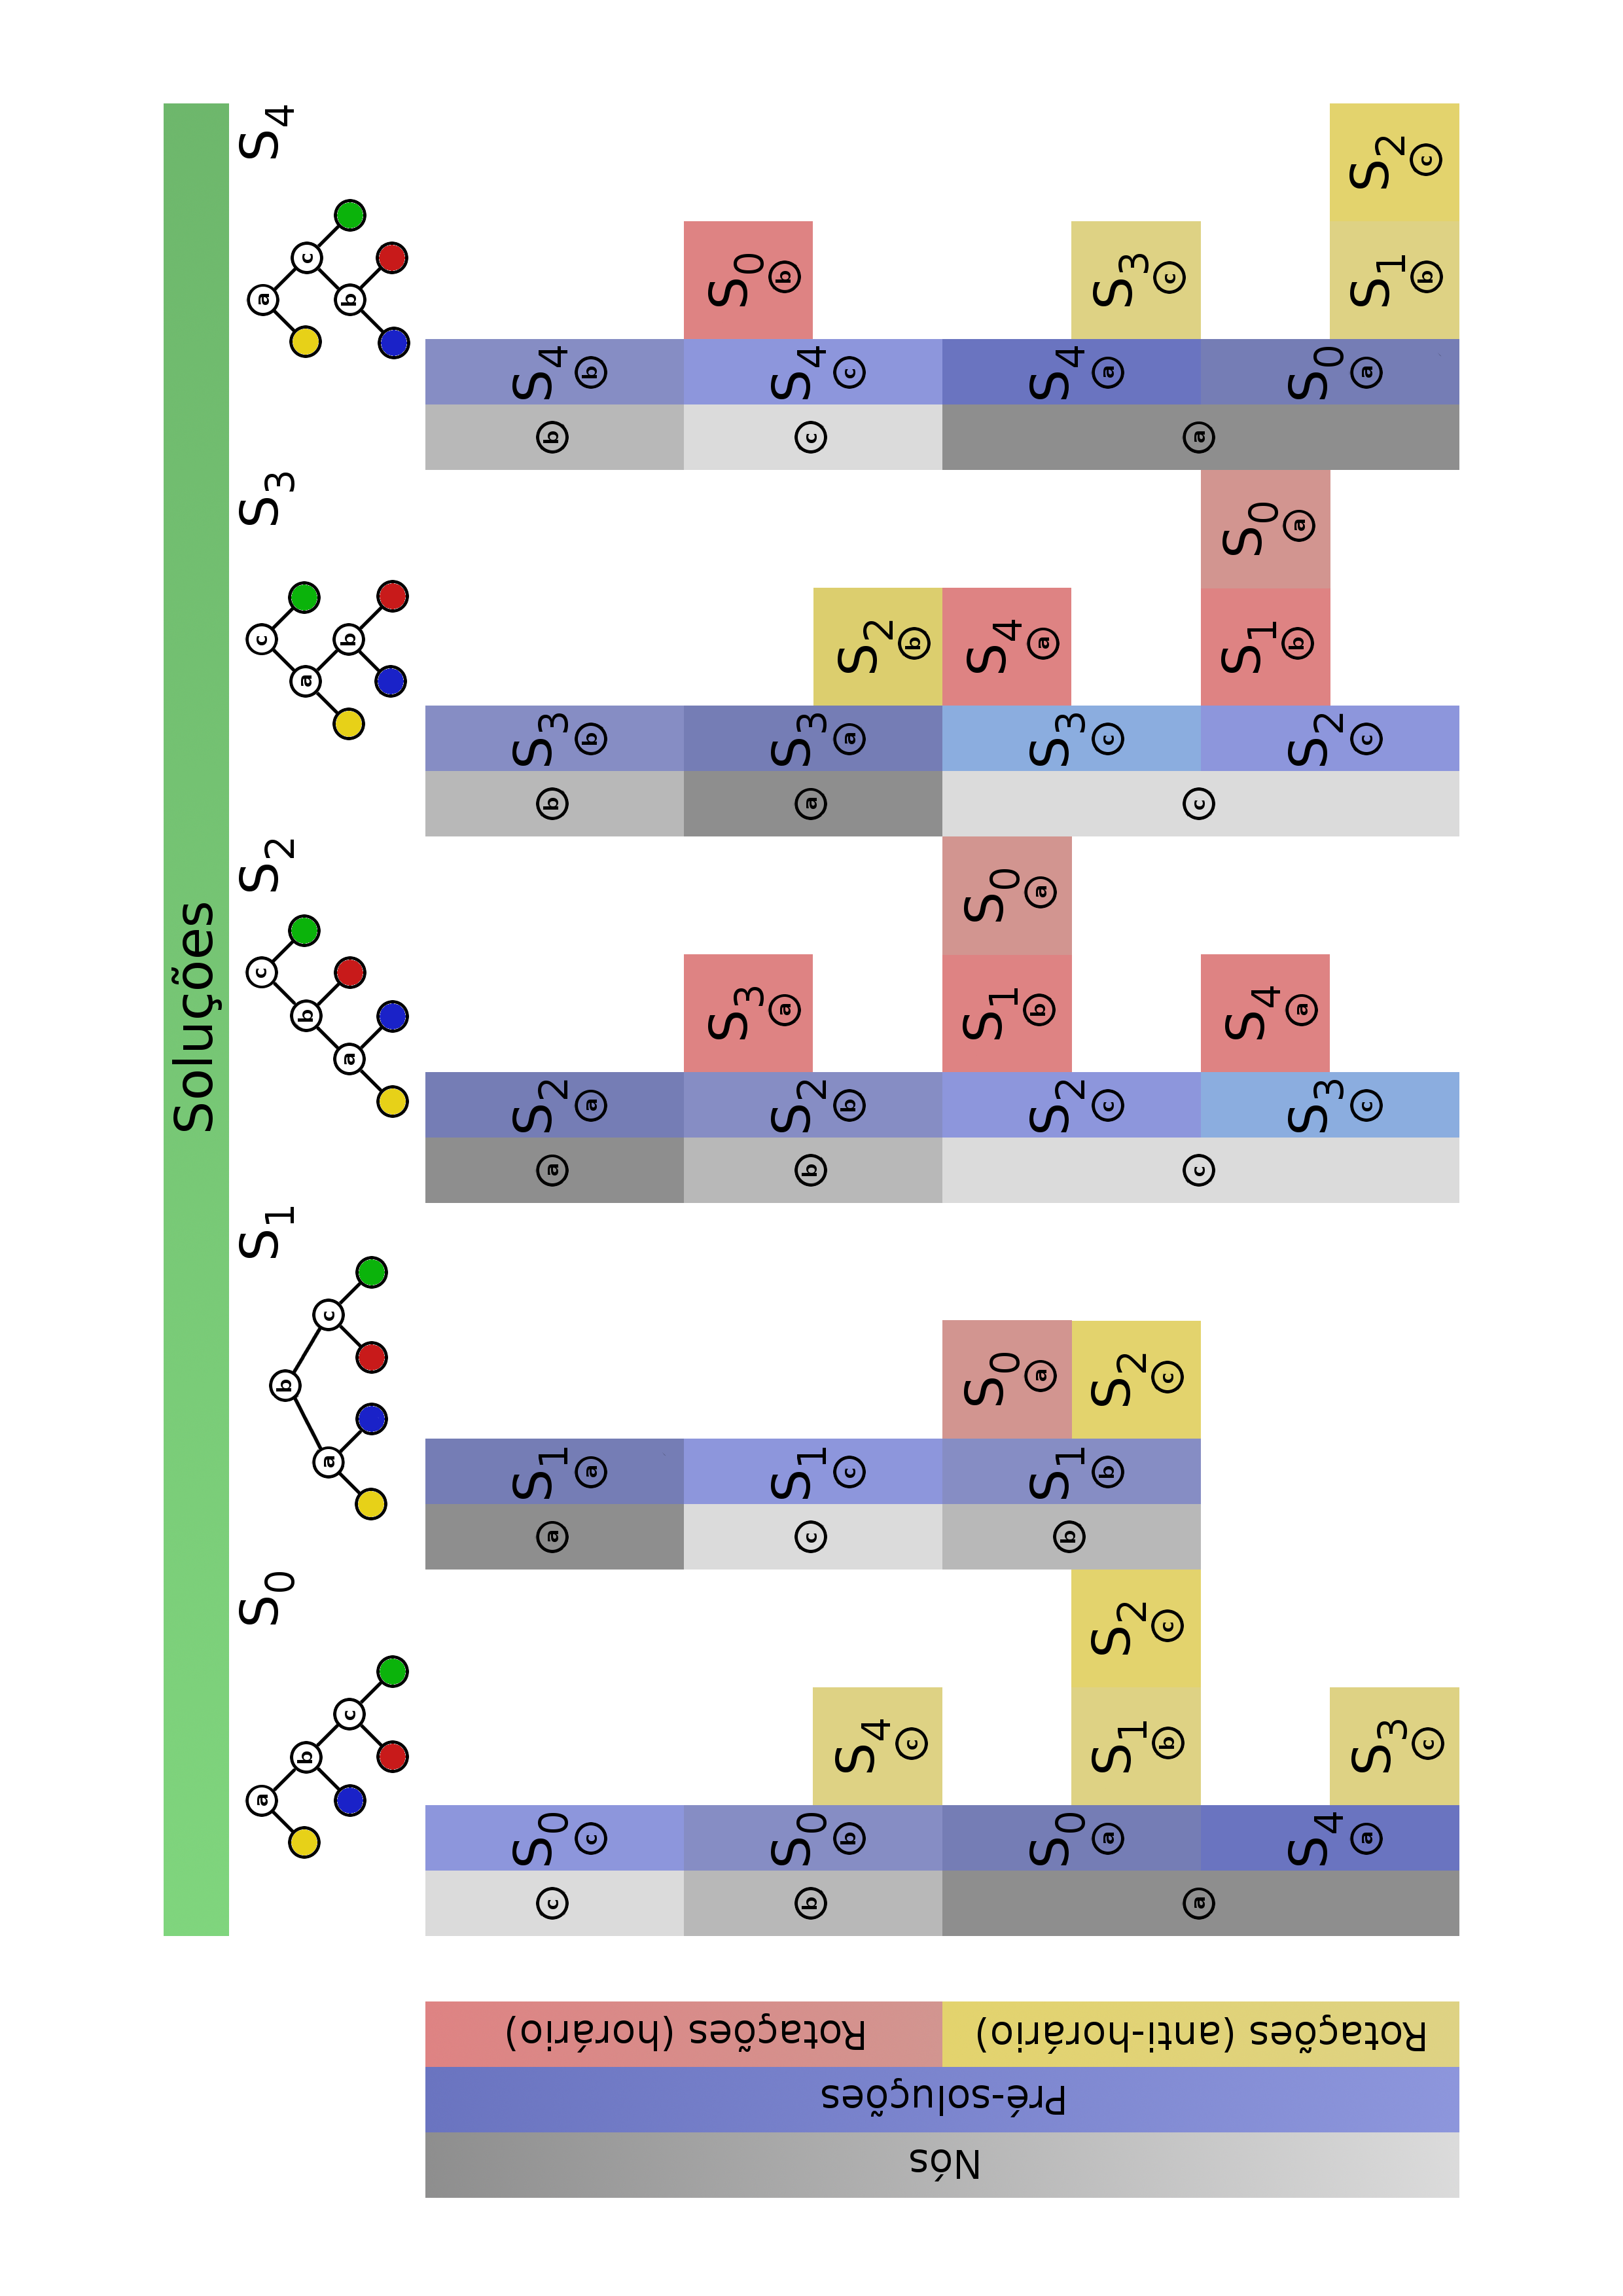
\includegraphics[scale=0.75]{alg_exp.png}
	\end{center}
% 	\legend{Fonte: Produzido pelo autor}
\end{figure}

\chapter{Gráfico: Tempos de execução do algoritmo de avaliação de soluções (escala linear)}

\begin{figure}[H]
	\begin{center}
	    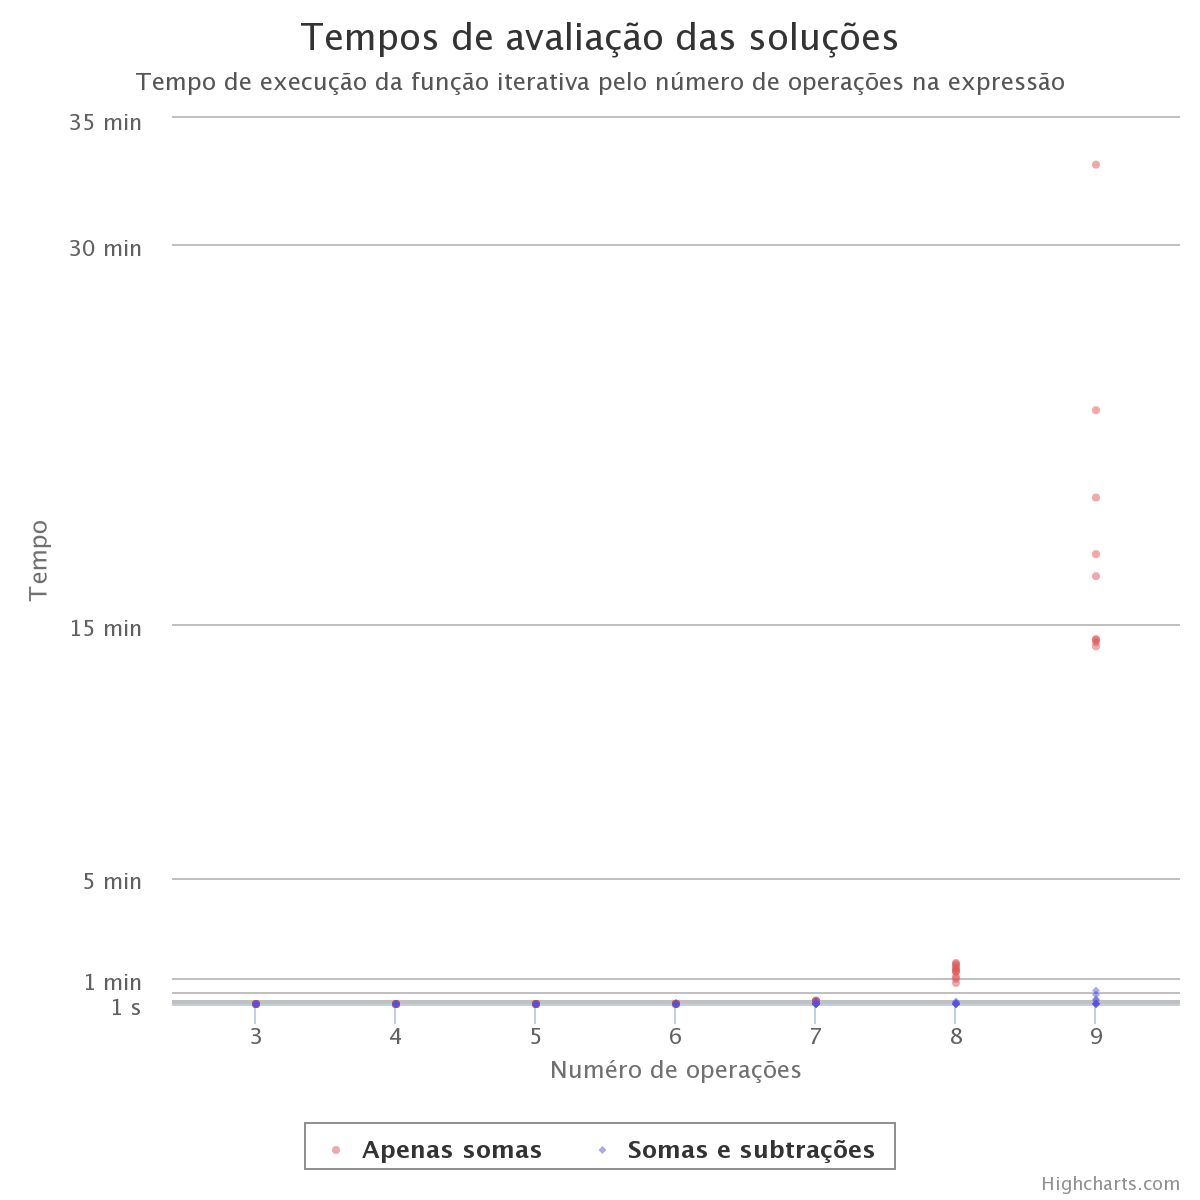
\includegraphics[scale=0.75]{timming_test_lin.png}
	\end{center}
\end{figure}

\chapter{Gráfico: Tempos de execução do algoritmo de avaliação de soluções (escala logarítmica)}

\begin{figure}[H]
	\begin{center}
	    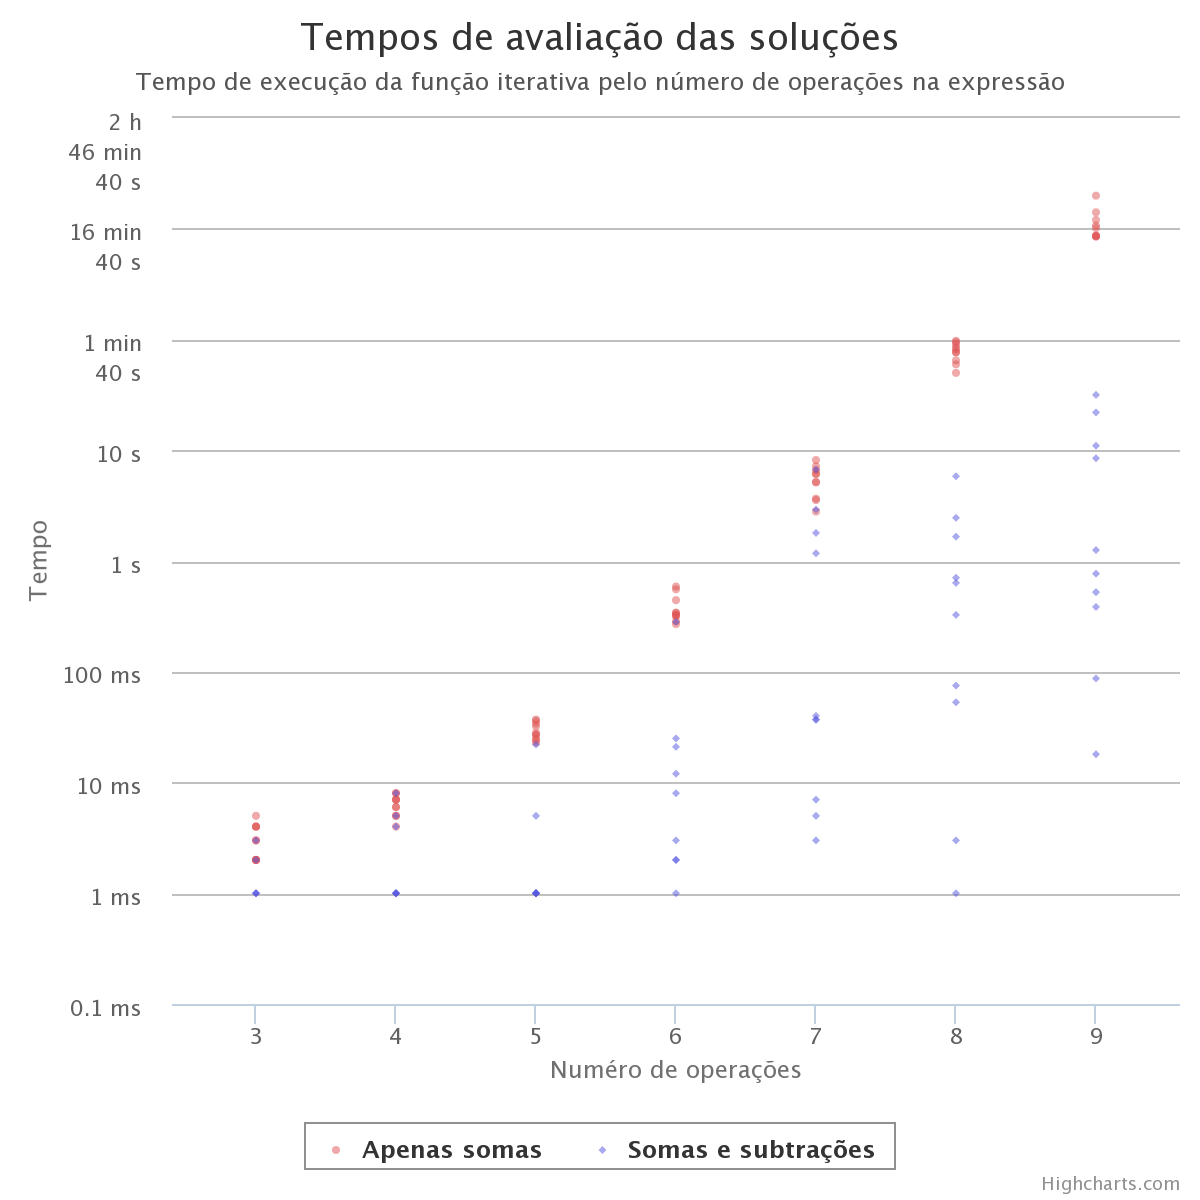
\includegraphics[scale=0.75]{timming_test_log.png}
	\end{center}
\end{figure}

\end{anexosenv}

\begin{anexosenv}

% Imprime uma página indicando o início dos anexos
\partanexos

% ---
\chapter{Pseudocódigo}

\begin{figure}[H]
	\begin{center}
	    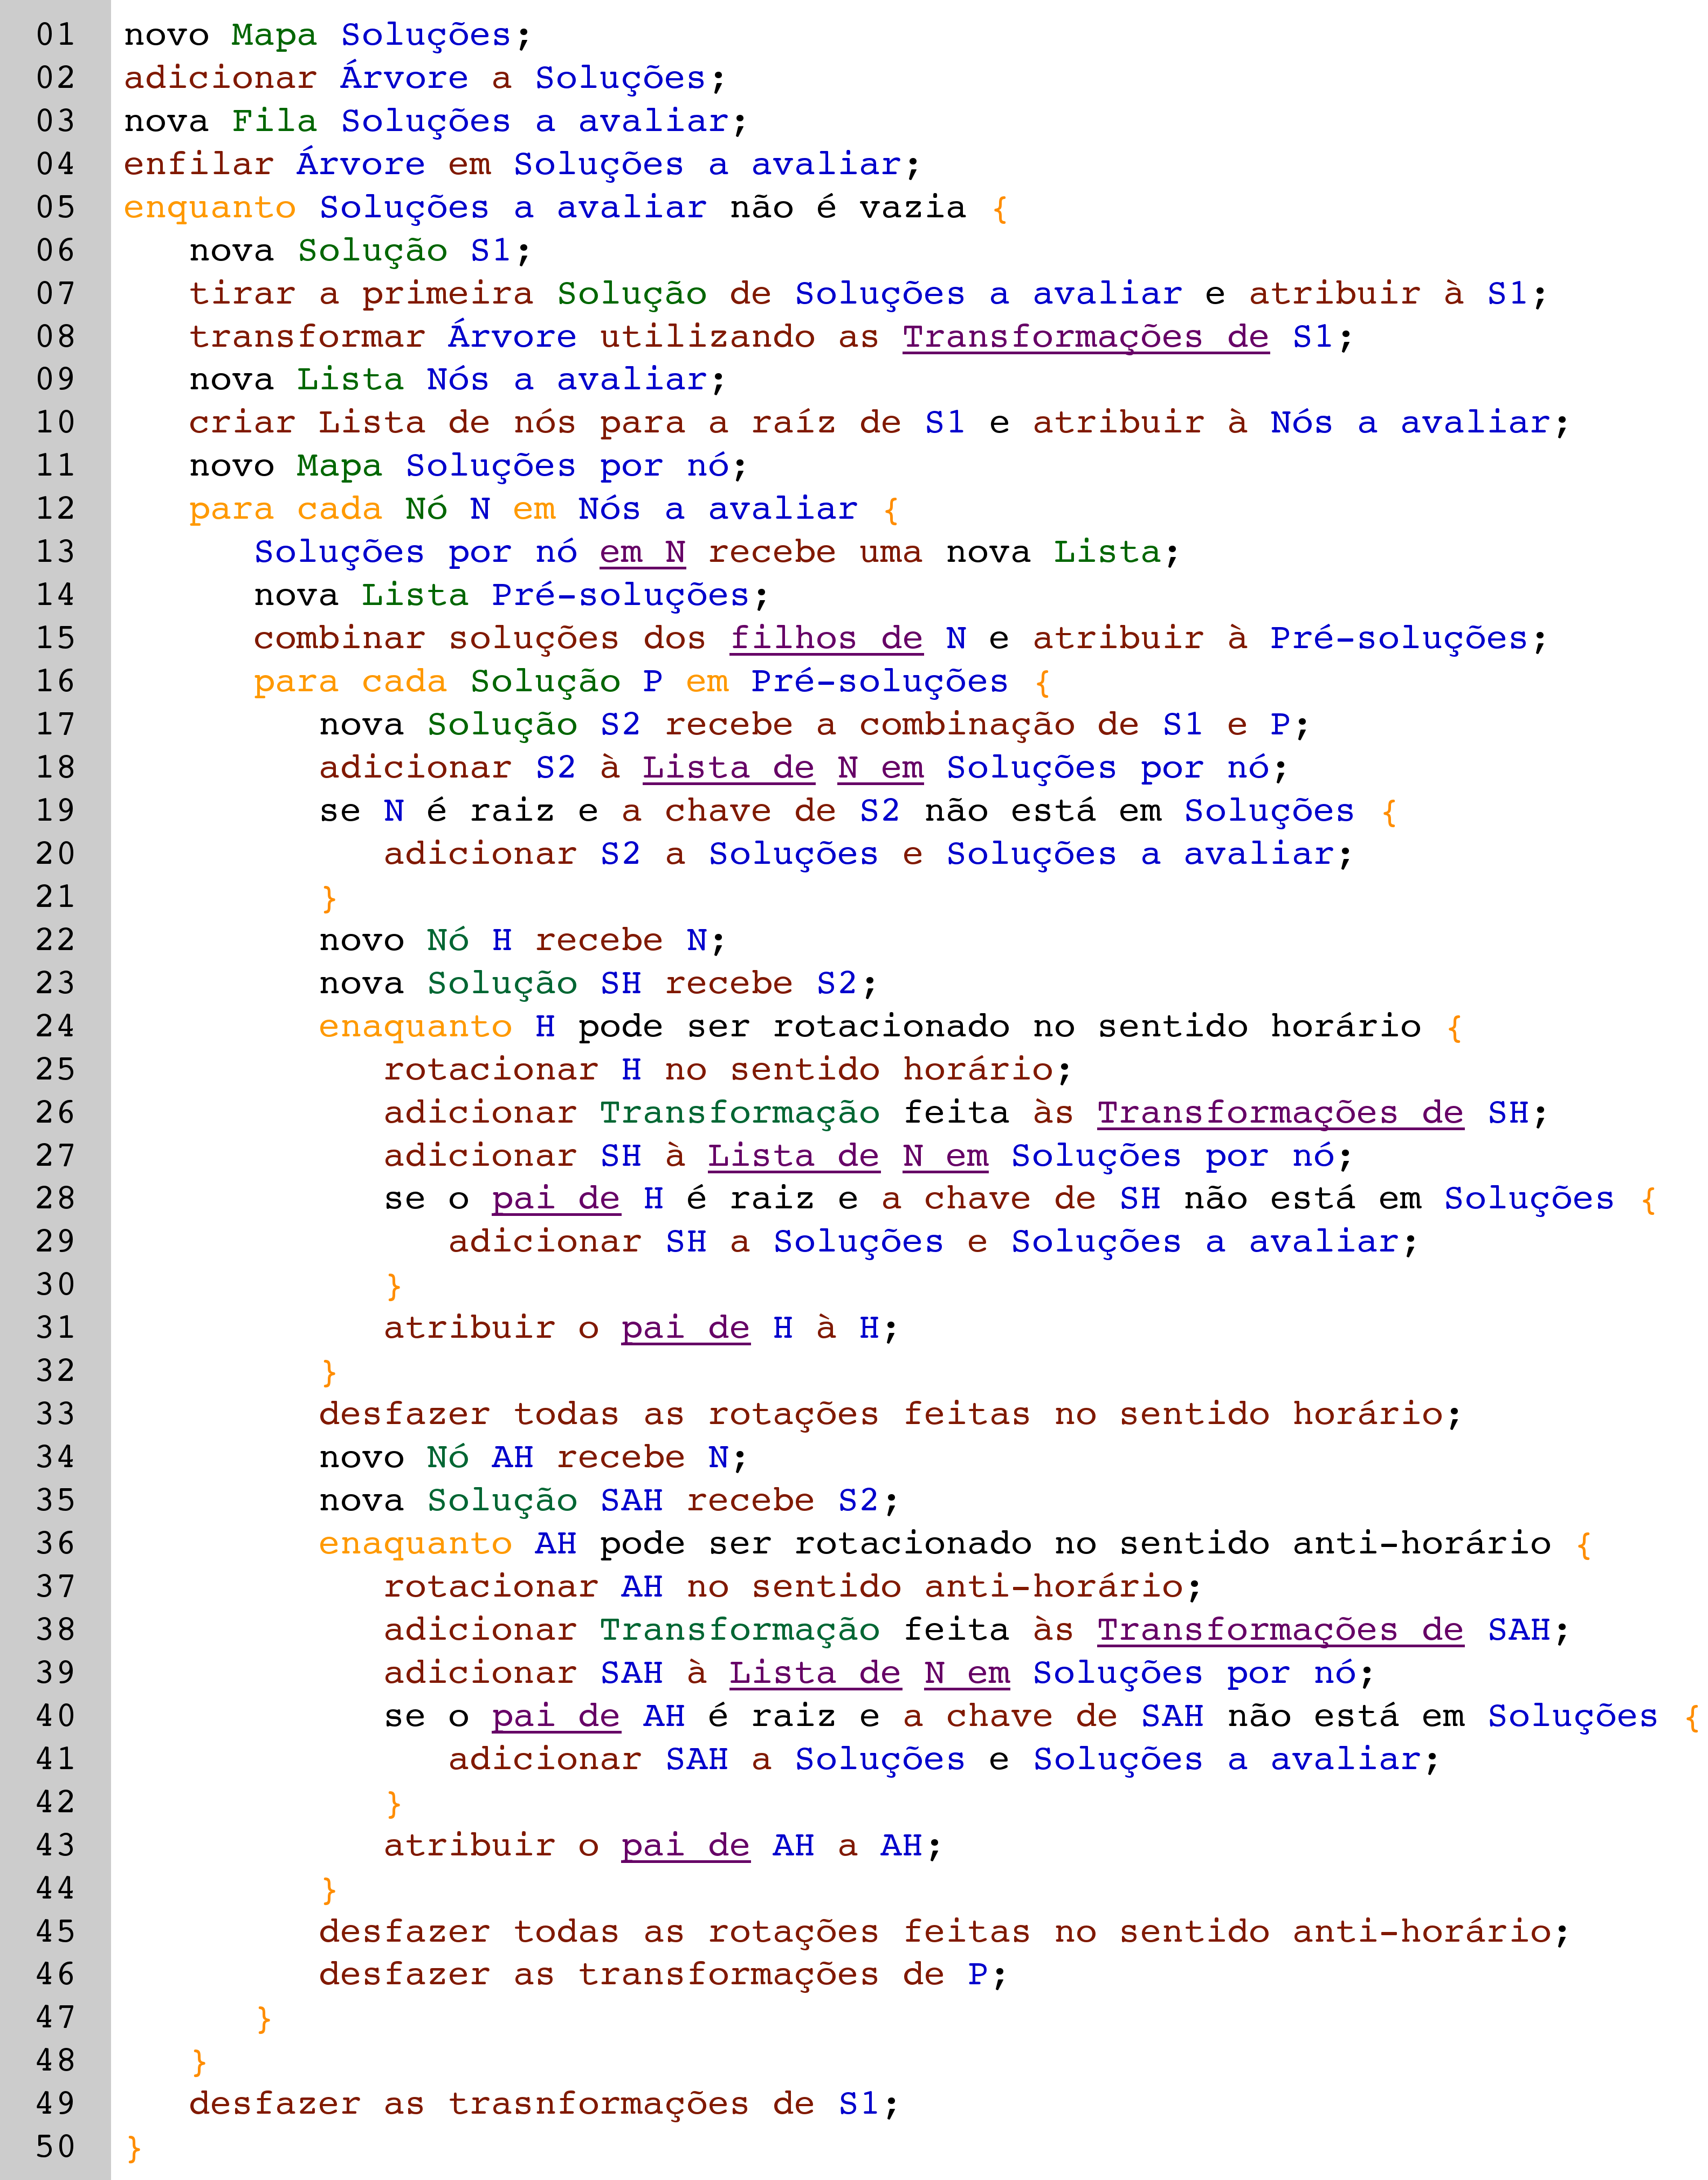
\includegraphics[scale=0.145]{psc.png}
	\end{center}
\end{figure}

\chapter{Exemplo: mapa de execução}

\begin{figure}[H]
% 	\caption{\label{gram_cls}Classes da Classificação de Chomsky e sua hierarquia}
	\begin{center}
	    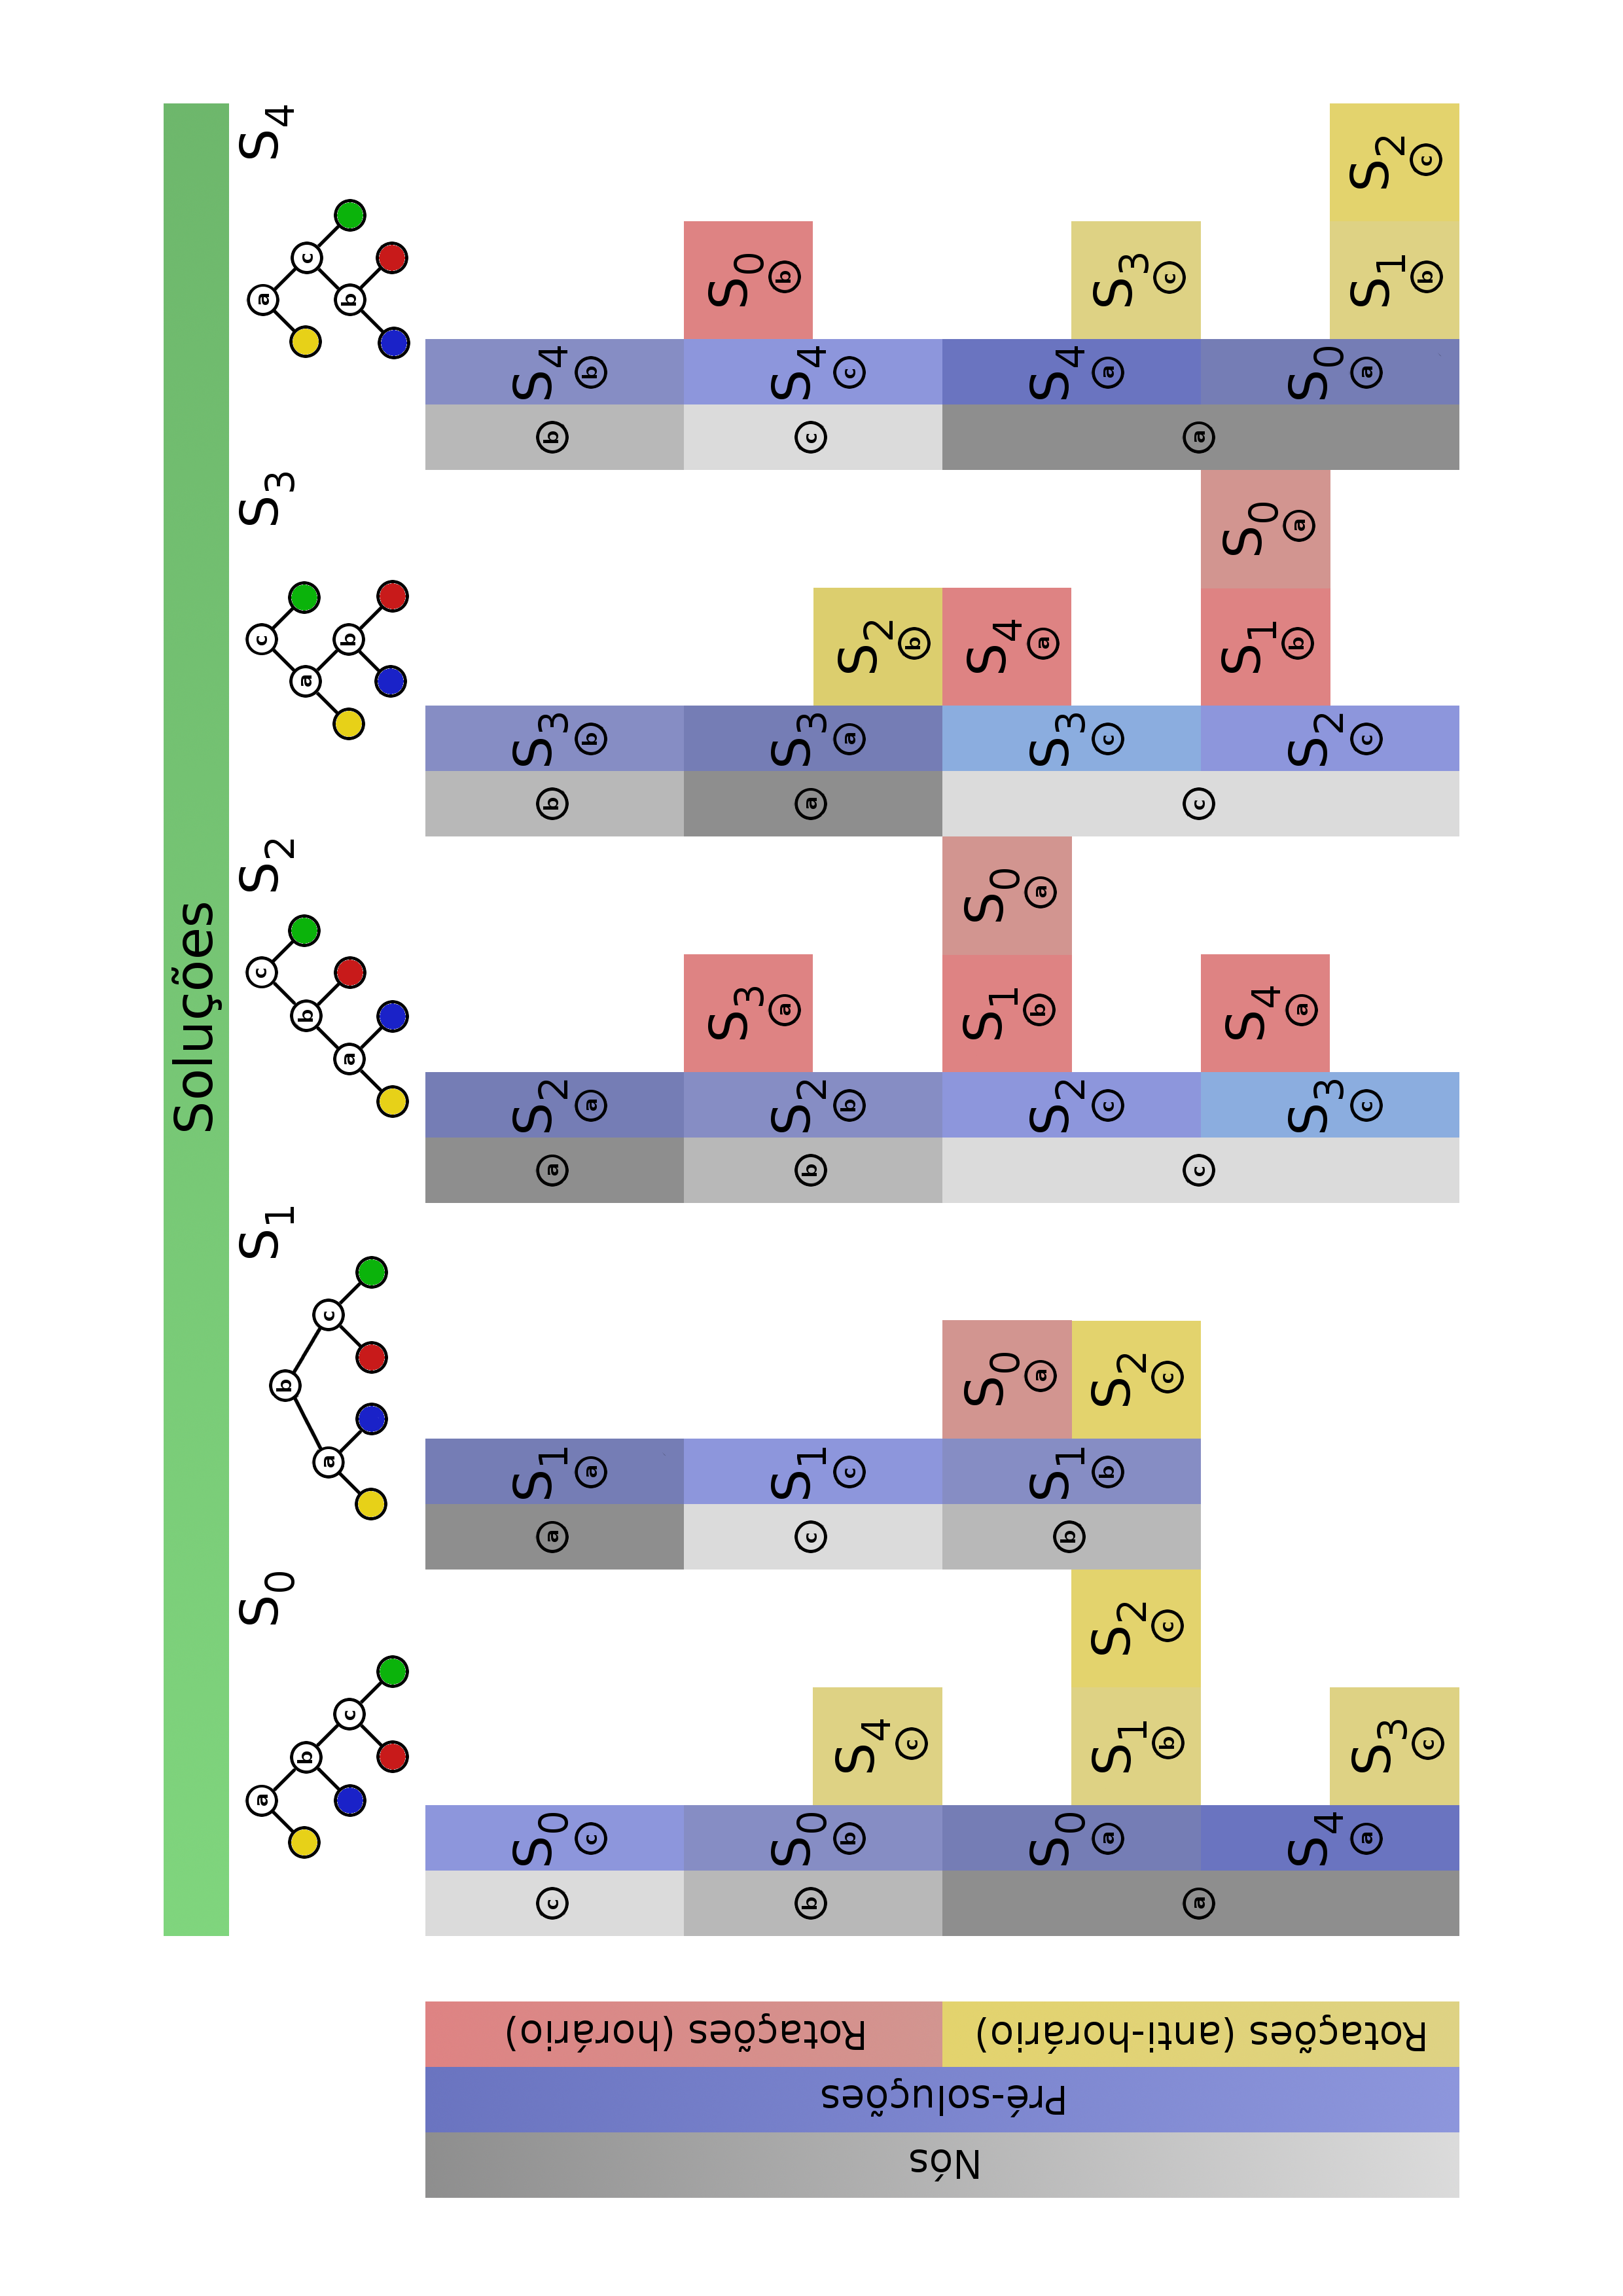
\includegraphics[scale=0.86]{alg_exp.png}
	\end{center}
% 	\legend{Fonte: Produzido pelo autor}
\end{figure}

\chapter{Gráfico: Tempos de execução do algoritmo de avaliação de soluções (escala linear)}

\begin{figure}[H]
	\begin{center}
	    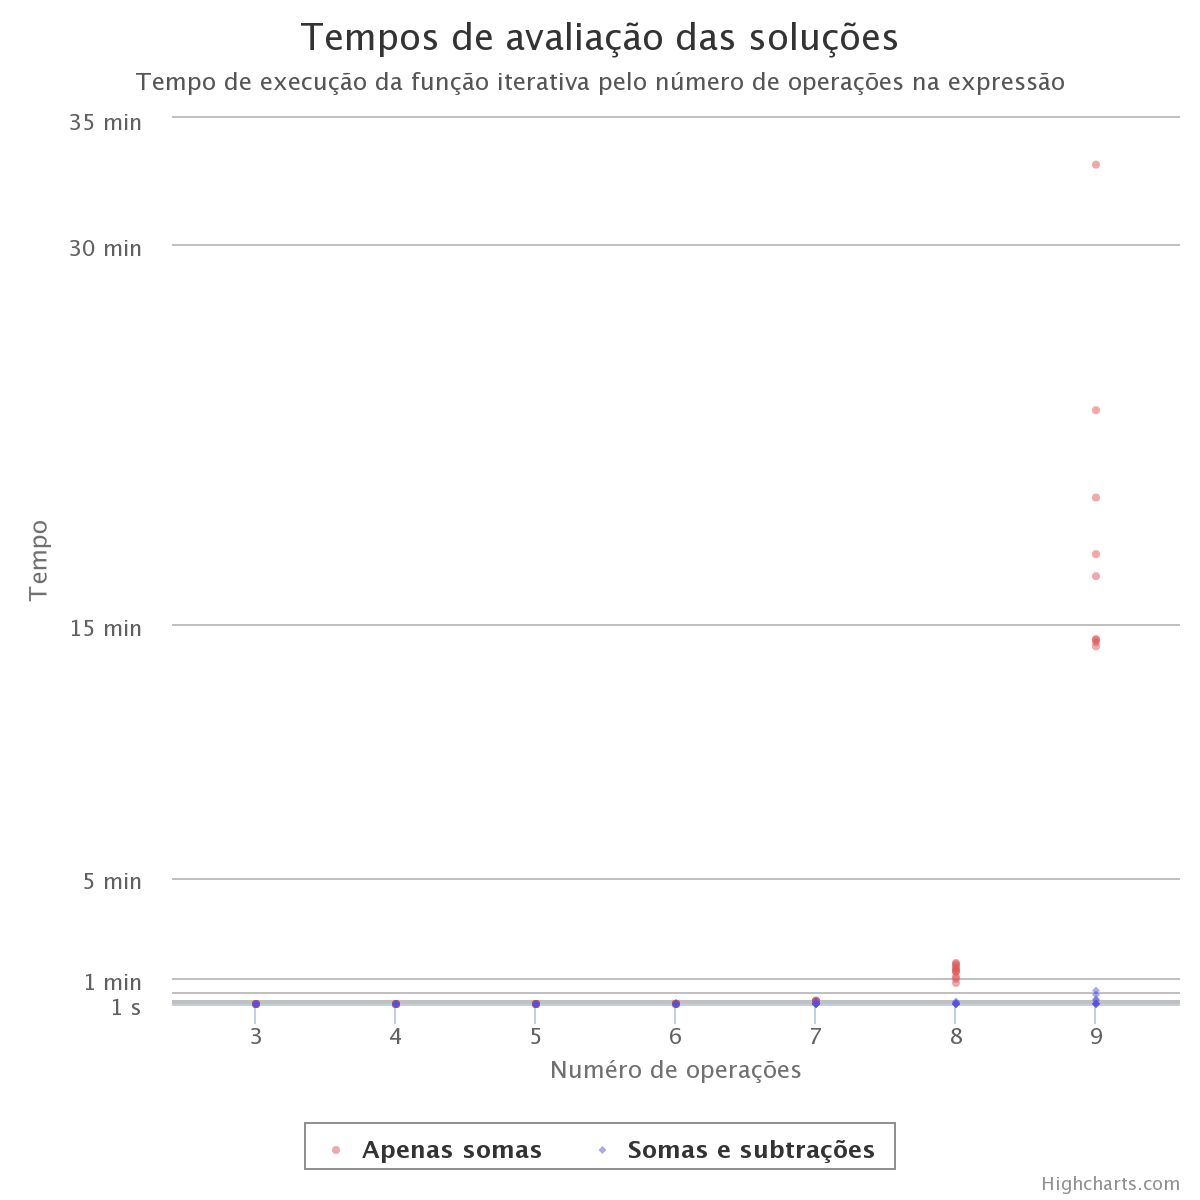
\includegraphics[scale=0.38]{timming_test_lin.png}
	\end{center}
\end{figure}

\chapter{Gráfico: Tempos de execução do algoritmo de avaliação de soluções (escala logarítmica)}

\begin{figure}[H]
	\begin{center}
	    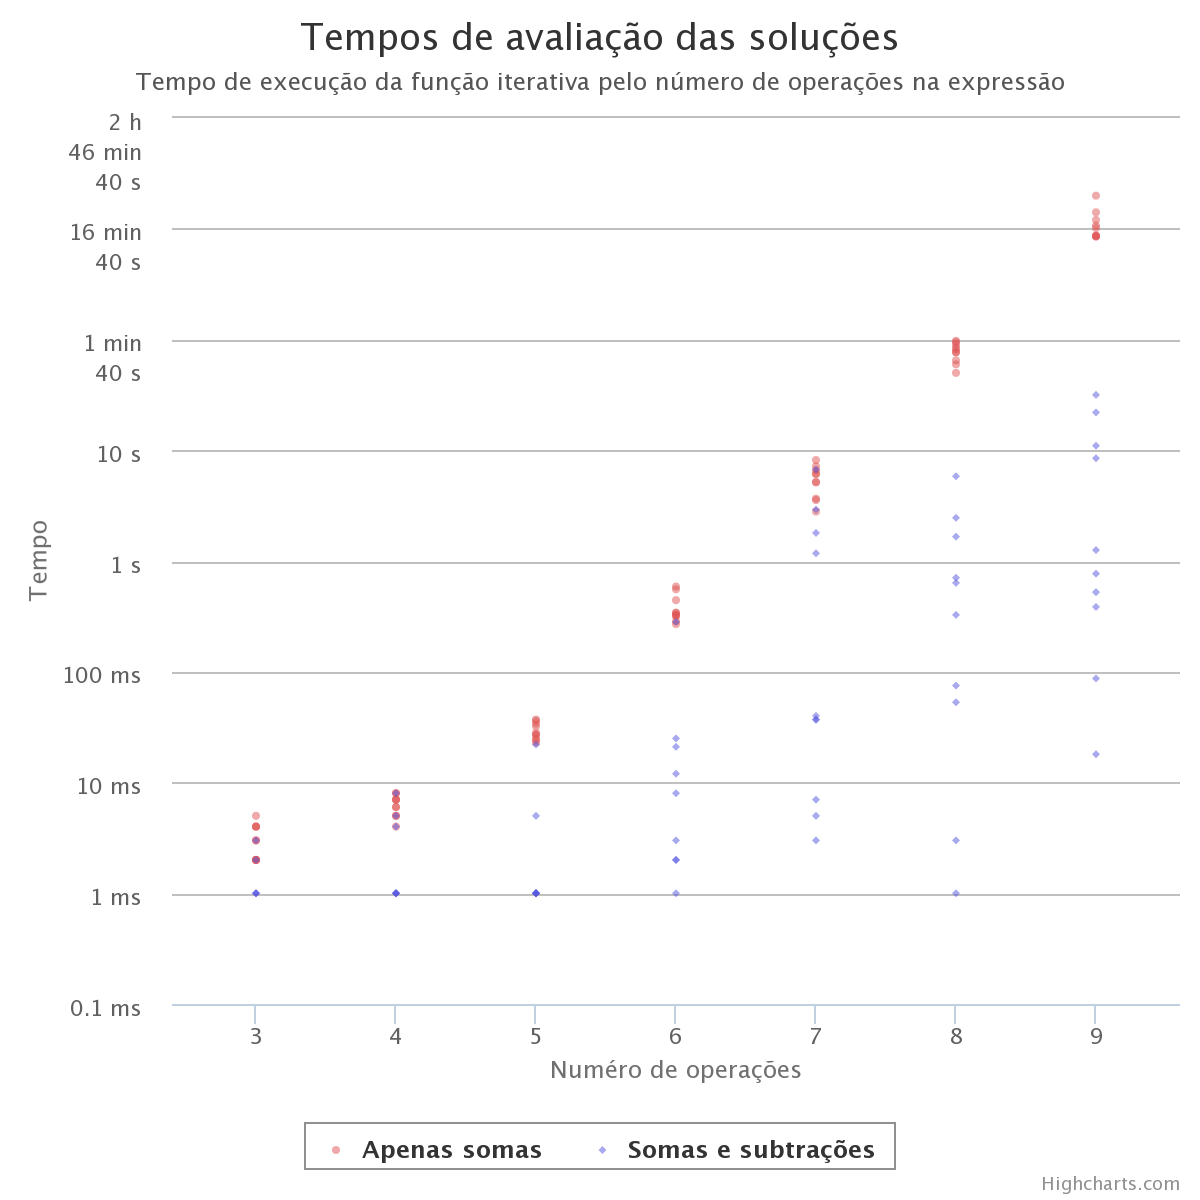
\includegraphics[scale=0.38]{timming_test_log.png}
	\end{center}
\end{figure}

\end{anexosenv}

%---------------------------------------------------------------------
% INDICE REMISSIVO
%---------------------------------------------------------------------
\phantompart
\printindex
%---------------------------------------------------------------------

\end{document}
